% !TEX options=--shell-escape

\documentclass[t, compress, mathserif, 10pt, xcolor=dvipsnames, table, aspectratio=43]{beamer}
%!TEX root = ./slides.tex

% Packages --------------------------------------------------------------------
\usepackage[T1]{fontenc}
\usepackage[utf8]{inputenc}
% \usepackage[frenchb]{babel}
\usepackage[english]{babel}
\usepackage{eulervm}
\usepackage{etoolbox,refcount}
\usepackage[normalem]{ulem} % strikeout with \sout{}
\usepackage{booktabs}
\usepackage{multirow}
\usepackage{multicol}
\usepackage{makecell}
\usepackage{pgfplots}
\usepackage{tikz}
\usepackage{environ}
\usepackage{circuitikz}
\usepackage{tikz-timing} % package pour les chronogrammes
\usepackage{caption}
\usepackage{graphicx}
\usepackage[export]{adjustbox} % align in includegraphics
\usepackage{stmaryrd} % llbracket
\usepackage{amsmath}
\usepackage{amssymb}
\usepackage{marvosym} % grosse fleche
\usepackage{calc}
\usepackage[english,onelanguage,ruled,linesnumbered,vlined]{algorithm2e}
\usepackage{bm}
\usepackage{pifont}
\usepackage{minted} % beautiful source code
\usepackage{tcolorbox}
\usepackage{etoolbox}
\usepackage{appendixnumberbeamer} % do not count backup slides in the page counter
\usepackage[
  labelnumber  = true,
  backend      = biber,
  sorting      = none,
  % style        = alphabetic,
  % citestyle    = alphabetic,
  maxnames     = 6,
  defernumbers = true,
  isbn         = false,
  doi          = true,
  url          = true,
  backref      = true]{biblatex}
\addbibresource{../tail/bibliography.bib}

% Parameters ------------------------------------------------------------------
% \renewcommand{\scriptsize}{\fontsize{5}{6}}
\renewcommand{\footnotesize}{\fontsize{7}{8.4}}
% % \renewcommand{\footnotesize}{\scriptsize}

\pgfplotsset{compat=newest}
\usepgfplotslibrary{colorbrewer}
\usepgfplotslibrary{groupplots}
\usetikzlibrary{matrix, positioning, fit, patterns, shapes, arrows, shapes.multipart, decorations.pathmorphing, calc, spy}

\tikzset{
    invisible/.style={opacity=0},
    visible on/.style={alt={#1{}{invisible}}},
    alt/.code args={<#1>#2#3}{%
      \alt<#1>{\pgfkeysalso{#2}}{\pgfkeysalso{#3}} % \pgfkeysalso doesn't change the path
    },
    hatch distance/.store in=\hatchdistance,
    hatch distance=7pt,
    hatch thickness/.store in=\hatchthickness,
    hatch thickness=0.5pt,
}
% \SetAlFnt{\footnotesize}
\AtBeginEnvironment{frame}{\setcounter{footnote}{0}}

% package 'minted'
\setminted{bgcolor=marronUni,fontsize=\fontsize{8}{9.2},tabsize=4,numbers=left,framesep=0pt,numbersep=2pt,xleftmargin=3.5mm,xrightmargin=3.5mm,highlightcolor=marronUni!90} % package 'minted'
\usemintedstyle{monokai} % friendly fruity
% https://tex.stackexchange.com/questions/252263/alignment-of-minted-line-numbers
% \newlength{\mintednumbersep}
% \AtBeginDocument{%
%   \sbox0{\tiny00}%
%   \setlength\mintednumbersep{\parindent}%
%   \addtolength\mintednumbersep{-\wd0}%
% }
\BeforeBeginEnvironment{minted}{\begin{tcolorbox}[colback=marronUni, colframe=black, arc=0.5mm, boxsep=0mm, boxrule=0.0mm, left=0mm, right=0mm, top=0mm, bottom=0mm]}
\AfterEndEnvironment{minted}{\end{tcolorbox}}
\renewcommand{\theFancyVerbLine}{\textcolor[rgb]{1,1,1}{\tiny{\arabic{FancyVerbLine}}}}
% \renewcommand{\theFancyVerbLine}{\sffamily\textcolor[rgb]{1,1,1}{\footnotesize\oldstylenums{\arabic{FancyVerbLine}}}}

% new shapes for pgfplot
\makeatletter
\pgfdeclarepatternformonly[\hatchdistance,\hatchthickness]{flexible hatch north east}
{\pgfqpoint{0pt}{0pt}}
{\pgfqpoint{\hatchdistance}{\hatchdistance}}
{\pgfpoint{\hatchdistance-1pt}{\hatchdistance-1pt}}%
{
    \pgfsetcolor{\tikz@pattern@color}
    \pgfsetlinewidth{\hatchthickness}
    \pgfpathmoveto{\pgfqpoint{0pt}{0pt}}
    \pgfpathlineto{\pgfqpoint{\hatchdistance}{\hatchdistance}}
    \pgfusepath{stroke}
}
\makeatletter
\pgfdeclarepatternformonly[\hatchdistance,\hatchthickness]{flexible hatch north west}
{\pgfqpoint{0pt}{0pt}}
{\pgfqpoint{\hatchdistance}{\hatchdistance}}
{\pgfpoint{\hatchdistance-1pt}{\hatchdistance-1pt}}%
{
    \pgfsetcolor{\tikz@pattern@color}
    \pgfsetlinewidth{\hatchthickness}
    \pgfpathmoveto{\pgfqpoint{\hatchdistance}{0pt}}
    \pgfpathlineto{\pgfqpoint{0pt}{\hatchdistance}}
    \pgfusepath{stroke}
}

\setbeamertemplate{caption}{\raggedright\insertcaption\par}

% biblatex
% separate multi-citations by a comma instead of a semicolon in 'biblatex'
\renewcommand*{\multicitedelim}{\addcomma\addspace}
% \renewcommand\mkbibacro[1]{{\footnotesize\MakeUppercase{#1}}}
\definecolor{bluecite}{HTML}{009DE0}
\setbeamertemplate{bibliography item}{\textcolor{black}{\insertbiblabel}}
\newcommand{\enumcite}[1]{{{\fontsize{6}{7.2}\selectfont \cite{#1}\quad \fullcite{#1}}}}

% package 'hyperref'
\hypersetup{
  colorlinks,
  allcolors=.,
  citecolor= bluecite,
  urlcolor=bluecite,
}
% package 'url'
\urlstyle{tt}


\SetKwComment{Comment}{$\triangleright$\ }{} % package 'algorithm2e'
\newcommand\mycommfont[1]{\small\ttfamily\textcolor{Comment}{#1}} % package 'algorithm2e'
\SetCommentSty{mycommfont} % package 'algorithm2e'


% Beamer template -------------------------------------------------------------
\usepackage{color}

\definecolor{Comment}{RGB}{97,161,176}

\definecolor{btfGreen}{RGB}{51,160,44}
\definecolor{btfRed}{RGB}{190,60,90}

\definecolor{bleuUni}{RGB}{0, 157, 224}
\definecolor{marronUni}{RGB}{68, 58, 49}
\definecolor{grayMarronUni}{RGB}{60, 60, 60}
\definecolor{grayBleuUni}{RGB}{118, 118, 118}

\definecolor{bluecite}{HTML}{009DE0}

\definecolor{Paired-2}{RGB}{166,206,227}
\definecolor{Paired-1}{RGB}{31,120,180}
\definecolor{Paired-4}{RGB}{178,223,138}
\definecolor{Paired-3}{RGB}{51,160,44}
\definecolor{Paired-6}{RGB}{251,154,153}
\definecolor{Paired-5}{RGB}{227,26,28}
\definecolor{Paired-8}{RGB}{253,191,111}
\definecolor{Paired-7}{RGB}{255,127,0}
\definecolor{Paired-10}{RGB}{202,178,214}
\definecolor{Paired-9}{RGB}{106,61,154}
\definecolor{Paired-12}{RGB}{255,255,153}
\definecolor{Paired-11}{RGB}{177,89,40}
\definecolor{Accent-1}{RGB}{127,201,127}
\definecolor{Accent-2}{RGB}{190,174,212}
\definecolor{Accent-3}{RGB}{253,192,134}
\definecolor{Accent-4}{RGB}{255,255,153}
\definecolor{Accent-5}{RGB}{56,108,176}
\definecolor{Accent-6}{RGB}{240,2,127}
\definecolor{Accent-7}{RGB}{191,91,23}
\definecolor{Accent-8}{RGB}{102,102,102}
\definecolor{Spectral-1}{RGB}{158,1,66}
\definecolor{Spectral-2}{RGB}{213,62,79}
\definecolor{Spectral-3}{RGB}{244,109,67}
\definecolor{Spectral-4}{RGB}{253,174,97}
\definecolor{Spectral-5}{RGB}{254,224,139}
\definecolor{Spectral-6}{RGB}{255,255,191}
\definecolor{Spectral-7}{RGB}{230,245,152}
\definecolor{Spectral-8}{RGB}{171,221,164}
\definecolor{Spectral-9}{RGB}{102,194,165}
\definecolor{Spectral-10}{RGB}{50,136,189}
\definecolor{Spectral-11}{RGB}{94,79,162}
\definecolor{Set1-1}{RGB}{228,26,28}
\definecolor{Set1-2}{RGB}{55,126,184}
\definecolor{Set1-3}{RGB}{77,175,74}
\definecolor{Set1-4}{RGB}{152,78,163}
\definecolor{Set1-5}{RGB}{255,127,0}
\definecolor{Set1-6}{RGB}{255,255,51}
\definecolor{Set1-7}{RGB}{166,86,40}
\definecolor{Set1-8}{RGB}{247,129,191}
\definecolor{Set1-9}{RGB}{153,153,153}
\definecolor{Set2-1}{RGB}{102,194,165}
\definecolor{Set2-2}{RGB}{252,141,98}
\definecolor{Set2-3}{RGB}{141,160,203}
\definecolor{Set2-4}{RGB}{231,138,195}
\definecolor{Set2-5}{RGB}{166,216,84}
\definecolor{Set2-6}{RGB}{255,217,47}
\definecolor{Set2-7}{RGB}{229,196,148}
\definecolor{Set2-8}{RGB}{179,179,179}
\definecolor{Dark2-1}{RGB}{27,158,119}
\definecolor{Dark2-2}{RGB}{217,95,2}
\definecolor{Dark2-3}{RGB}{117,112,179}
\definecolor{Dark2-4}{RGB}{231,41,138}
\definecolor{Dark2-5}{RGB}{102,166,30}
\definecolor{Dark2-6}{RGB}{230,171,2}
\definecolor{Dark2-7}{RGB}{166,118,29}
\definecolor{Dark2-8}{RGB}{102,102,102}
\definecolor{Reds-1}{RGB}{255,245,240}
\definecolor{Reds-2}{RGB}{254,224,210}
\definecolor{Reds-3}{RGB}{252,187,161}
\definecolor{Reds-4}{RGB}{252,146,114}
\definecolor{Reds-5}{RGB}{251,106,74}
\definecolor{Reds-6}{RGB}{239,59,44}
\definecolor{Reds-7}{RGB}{203,24,29}
\definecolor{Reds-8}{RGB}{165,15,21}
\definecolor{Reds-9}{RGB}{103,0,13}
\definecolor{Greens-1}{RGB}{247,252,245}
\definecolor{Greens-2}{RGB}{229,245,224}
\definecolor{Greens-3}{RGB}{199,233,192}
\definecolor{Greens-4}{RGB}{161,217,155}
\definecolor{Greens-5}{RGB}{116,196,118}
\definecolor{Greens-6}{RGB}{65,171,93}
\definecolor{Greens-7}{RGB}{35,139,69}
\definecolor{Greens-8}{RGB}{0,109,44}
\definecolor{Greens-9}{RGB}{0,68,27}
\definecolor{Blues-1}{RGB}{247,251,255}
\definecolor{Blues-2}{RGB}{222,235,247}
\definecolor{Blues-3}{RGB}{198,219,239}
\definecolor{Blues-4}{RGB}{158,202,225}
\definecolor{Blues-5}{RGB}{107,174,214}
\definecolor{Blues-6}{RGB}{66,146,198}
\definecolor{Blues-7}{RGB}{33,113,181}
\definecolor{Blues-8}{RGB}{8,81,156}
\definecolor{Blues-9}{RGB}{8,48,107}

\usecolortheme[named=bleuUni]{structure}

% Special commands : ddfrac and actionenv and compresslist
\newcommand\ddfrac[2]{\frac{\displaystyle #1}{\displaystyle #2}}

\newenvironment<>{varblock}[2][\textwidth]{%
  \setlength{\textwidth}{#1}
  \begin{actionenv}#3%
    \def\insertblocktitle{#2}%
    \par%
    \usebeamertemplate{block begin}}
  {\par%
    \usebeamertemplate{block end}%
  \end{actionenv}}

\newcommand{\compresslist}{ % Define a command to reduce spacing within itemize/enumerate environments, this is used right after \begin{itemize} or \begin{enumerate}
\setlength{\itemsep}{1pt}
\setlength{\parskip}{0pt}
\setlength{\parsep}{0pt}
}

\newcommand*\circled[1]{\tikz[baseline=(char.base)]{%
      \node[shape=circle,fill=bleuUni,inner sep=2pt] (char) {\textbf{\textcolor{white}{#1}}};}}

\newcommand{\itmsp}[1] {\setlength\itemsep{#1}}
%%%%%%%%%%%%%%%%%%%%%%%%%

%%%%% Beamer
\usepackage[bars]{beamerthemetree} % Beamer theme v 2.2
\mode<presentation>
\newcommand*\oldmacro{}%
\let\oldmacro\insertshorttitle%
\renewcommand*\insertshorttitle{%
 \oldmacro\hspace{0pt plus 1 filll}%
\insertframenumber\,/\,\inserttotalframenumber}
\setbeamertemplate{footline}[frame number]
\setbeamersize{text margin left=10pt,text margin right=10pt}
\setbeamerfont{frametitle}{size=\small}
\setbeamertemplate{frametitle}{ \nointerlineskip %
\begin{beamercolorbox}[wd=\paperwidth,ht=2.2ex,dp=.9ex,left]{frametitle} %
                       \hspace*{2ex}\strut\bfseries\color{bleuUni!15!white}\insertframetitle\strut\par %
\end{beamercolorbox}}

%\setbeamerfont{headline}{size=\footnotesize}

% \usepackage{animate}
% \usepackage{multimedia}
\usetheme{Ilmenau} % Beamer theme v 3.0
\setbeamercolor{section in head/foot}{bg=marronUni}
\useinnertheme{circles} %rectangle bullet points instead of circle ones
\usepackage{beamerthemebars}
\beamertemplatenavigationsymbolsempty
%\setbeamercolor{navigation symbols dimmed}{fg=red!80!black}
%\setbeamercolor{navigation symbols}{fg=red!80!black}
%%%%%%%%%%%%%%%%%%%%%%%%%

\setbeamertemplate{headline}{%
\begin{beamercolorbox}[colsep=1.5pt]{upper separation line head}
\end{beamercolorbox}
\begin{beamercolorbox}{section in head/foot}
    \vskip2pt\insertsectionnavigationhorizontal{\paperwidth}{}{}\vskip2pt
\end{beamercolorbox}%
\begin{beamercolorbox}[ht=10pt]{subsection in head/foot}%
    \vskip2pt\insertsubsectionnavigationhorizontal{\paperwidth}{}{}\vskip2pt
\end{beamercolorbox}%
\begin{beamercolorbox}[colsep=1.5pt]{lower separation line head}
\end{beamercolorbox}
}

\setbeamertemplate{blocks}[rounded][shadow=false]

\AtBeginSection[]
{
\begin{frame}[c]{Organization of the Presentation}
  \tableofcontents[
      currentsection,
      subsectionstyle=hide,
  ]
\end{frame}
}

% MIPP ------------------------------------------------------------------------

\newcommand{\MIPP}{MIPP\xspace}
\newcommand{\longMIPP}{MyIntrinsics++\xspace}
\newcommand{\TSIMD}{T-SIMD\xspace}
\newcommand{\xsimd}{xsimd\xspace}
\newcommand{\simdpp}{simdpp\xspace}
\newcommand{\Vc}{Vc\xspace}
\newcommand{\VCL}{VCL\xspace}
\newcommand{\BoostSIMD}{Boost.SIMD\xspace}
\newcommand{\bSIMD}{bSIMD\xspace}
\newcommand{\AFFECT}{AFF3CT\xspace}

\newcommand{\C}{\texttt{C}\xspace}
\newcommand{\Cxx}{\texttt{C++}\xspace}
\newcommand{\Cxy}[1]{\texttt{C++{#1}}\xspace}
\newcommand{\CppUnit}{\texttt{CppUnit}\xspace}

\newcommand{\cmark}{\textcolor{btfGreen}{\ding{51}}}
\newcommand{\xmark}{\textcolor{btfRed}{\ding{55}}}
\newcommand{\Arikan}{Ar{\i}kan\xspace}

\DeclareMathOperator*{\sign}{sign}
\DeclareMathOperator*{\DecoderSC}{DecoderSC}
\DeclareMathOperator*{\hardDecide}{h_d}

% \newcommand{\highlight}[2]{\colorbox{#1}{\ensuremath{#2}}}

\newcommand{\highlight}[2][yellow]{\mathchoice%
  {{\setlength{\fboxsep}{0pt}\colorbox{#1}{$\displaystyle#2$}}}%
  {{\setlength{\fboxsep}{0pt}\colorbox{#1}{$\textstyle#2$}}}%
  {{\setlength{\fboxsep}{0pt}\colorbox{#1}{$\scriptstyle#2$}}}%
  {{\setlength{\fboxsep}{0pt}\colorbox{#1}{$\scriptscriptstyle#2$}}}}%

\newcommand{\R}{\textsuperscript{\textregistered}\xspace}
\newcommand{\TM}{\textsuperscript{\texttrademark}\xspace}

% add column types for big table
\newcolumntype{L}[1]{>{\raggedright\let\newline\\\arraybackslash\hspace{0pt}}m{#1}}
\newcolumntype{C}[1]{>{\centering\let\newline\\\arraybackslash\hspace{0pt}}m{#1}}
\newcolumntype{R}[1]{>{\raggedleft\let\newline\\\arraybackslash\hspace{0pt}}m{#1}}
\newlength{\simcolwidth}
\setlength{\simcolwidth}{0.5cm}

\title{\textbf{Optimization and Parallelization Methods \\%
               for the Software-defined Radio}}
\author[Adrien Cassagne\hspace{8.0925cm}{adrien.cassagne@u-bordeaux.fr}] {Adrien Cassagne}
\titlegraphic{
\includegraphics[height=.9cm]{../head/pic/inr_logo_rouge.png} \hfil %
              
\includegraphics[height=.9cm]{../head/pic/ims.png} \hfil %
              
\includegraphics[height=.9cm]{../head/pic/ub.jpg}}
\date{December 8, 2020}

\begin{document}

%!TEX root = ./slides.tex

% TikZ maccro -----------------------------------------------------------------
\newcommand{\Cloud}[3]{
\begin{scope}[shift={#1},scale=#3]
  \draw[fill=white] (-1.6,-0.7) .. controls (-2.3,-1.1)
  and (-2.7,0.3) .. (-1.7,0.3)coordinate(asy1) .. controls (-1.6,0.7)
  and (-1.2,0.9) .. (-0.8,0.7) .. controls (-0.5,1.5)
  and (0.6,1.3) .. (0.7,0.5) .. controls (1.5,0.4)
  and (1.2,-1) .. (0.4,-0.6)coordinate(asy2) .. controls (0.2,-1)
  and (-0.2,-1) .. (-0.5,-0.7) .. controls (-0.9,-1)
  and (-1.3,-1) .. cycle;
  \node at ($(asy1)!0.5!(asy2)$) {#2};
\end{scope}
}

\newcommand{\Phone}[3]{
\begin{scope}[shift={#1},scale=#2]
  \draw[black,rounded corners=1pt, thick, fill=white]  (0,0) rectangle (0.9,1.8);
  \draw[black, thick]  (0.7,1.8) -- (0.7,2.1);
\end{scope}
}

\newcommand{\PhoneGroup}[3]{
\begin{scope}[shift={#1},scale=#2]
  \Phone{(0,0)}{1.0};
  \Phone{(0.5,-0.5)}{1.0};
  \Phone{(0.2,-1.0)}{1.0};
\end{scope}
}

\newcommand{\SmartPhone}[3]{
\begin{scope}[shift={#1},scale=#2]
  \draw[black,rounded corners=1pt, thick, fill=white]  (0,0) rectangle (1.25,2);
  \draw[black,rounded corners=1pt]  (0.625-0.2, 0.10) rectangle (0.625+0.2,0.10+0.15);
\end{scope}
}

\newcommand{\SmartPhoneGroup}[3]{
\begin{scope}[shift={#1},scale=#2]
  \SmartPhone{(0,0)}{1.0};
  \SmartPhone{(0.8,-0.5)}{1.0};
  \SmartPhone{(0.2,-1.0)}{1.0};
\end{scope}
}

\newcommand{\thread}[3]{
  \begin{scope}[shift={#1},scale=#2]
    \draw[thick] plot [smooth,tension=0.7] coordinates {(0,1) (0.15,0.875) (-0.1,0.625) (0.2,0.25) (0,0)} node (#3){};
  \end{scope}
}

\newcommand{\Thread}[3]{
   \draw[thick, xshift=#1cm, yshift=#2cm] plot [smooth,tension=0.7] coordinates {(0,0.5) (0.075,0.4375) (-0.05,0.3125) (0.1,0.125) (0,0)} node (#3){};
}

\begin{frame}[c]
  \titlepage
\end{frame}

\section[Introduction]{Introduction \& Context}

\subsection[Introduction]{Introduction}

\begin{frame}{Introduction}
  \begin{figure}[htp]
  \centering
  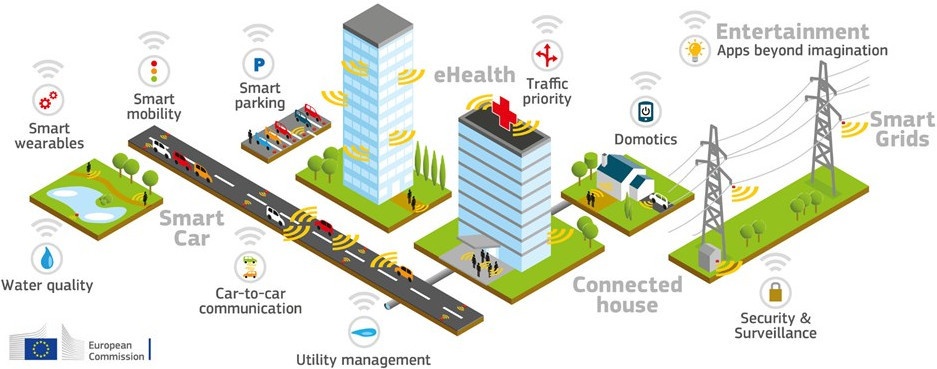
\includegraphics[scale=0.35]{pics/5G_crop}
\end{figure}
  \begin{itemize}
    \item Nowadays digital communication systems are everywhere
    \item Real-time systems are traditionally implemented in hardware
    \item Needs validation of more robust and more complex systems
    \item Needs to flexibility to adapt to many parameters
    \item New challenge: implement digital communication systems in software
      \\\vspace*{.5em}
      {\color{bleuUni}\Large\MVRightarrow} \textbf{Require high performance implementations}
  \end{itemize}
\end{frame}

\subsection[Applicative Contexts]{Applicative Contexts}

\begin{frame}{Digital Communication Systems}
  \begin{figure}[!h]
  \centering
  \begin{tikzpicture}[scale=0.65, every node/.style={transform shape}]
    \path[use as bounding box] (-2.2, -1.2) rectangle (11.8, 5.2);
    % \draw (-2.2, -1.2) rectangle (11.8, 5.2);

    \only<1>{
    \tikzset{ txt/.style={draw=white, rounded corners=0pt, minimum height=1cm, minimum width=2.5cm, text=white, align=center} }
    \tikzset{ rxt/.style={draw=white, rounded corners=0pt, minimum height=1cm, minimum width=2.5cm, text=white, align=center} }
    }
    \only<2->{
    \tikzset{ txt/.style={draw=Paired-1, rounded corners=0pt, minimum height=1cm, minimum width=2.5cm, text=Paired-1, align=center} }
    \tikzset{ rxt/.style={draw=Paired-3, rounded corners=0pt, minimum height=1cm, minimum width=2.5cm, text=Paired-3, align=center} }
    }
    \node[style={txt}] (sen) at (0,4) {Source\\Encoder};
    \node[style=txt] (enc) at (4,4) {Channel\\Encoder};
    \node[style=txt] (mod) at (8,4) {Digital\\Modulator};
    \Cloud{(11,2)}{}{0.65};
    \node[text=black] (chn) at (10.7,2) {Channel};
    \node[style=rxt] (dem) at (8,0) {Digital\\Demodulator};

    \node[style=rxt] (dec) at (4,0) {Channel\\Decoder};
    \node[style={rxt}] (sde) at (0,0) {Source\\Decoder};

    \only<1>{
    \node[draw=Paired-1, fill=Paired-1!20, rounded corners=2pt, minimum height=1.5cm, dashed, fit=(sen) (enc) (mod), align=center, label=center: {\large\textbf{Transmission chain}}] (tx) {};
    \node[draw=Paired-3, fill=Paired-3!20, rounded corners=2pt, minimum height=1.5cm, dashed, fit=(dem) (dec) (sde), align=center, label=center: {\large\textbf{Reception chain}}] (rx) {};
    }
    \only<2->{
    \node[draw=Paired-1, rounded corners=2pt, label={[Paired-1]below:Transmitter}, minimum height=1.5cm, dashed, fit=(sen) (enc) (mod)] (tx) {};
    \node[draw=Paired-3, rounded corners=2pt, label={[Paired-3]above:Receiver   }, minimum height=1.5cm, dashed, fit=(dem) (dec) (sde)] (rx) {};
    }

    \draw[<-,>=latex] (tx.west)  -- (-2,  4) node [left,    above           ] {$\bm{m}$};
    \draw[->,>=latex] (tx.east)  -- (10,  4) node [midway,  above           ] {$\bm{x}$};
    \draw[-         ] ( 9.9,4)   -- (10.5,4) node [antenna, above, scale=0.5] {};
    \draw[-         ] (10  ,0)   -- (10.5,0) node [antenna, above, scale=0.5] {};
    \draw[<-,>=latex] (rx.east)  -- (10,  0) node [midway,  above           ] {$\bm{y}$};
    \draw[->,>=latex] (rx.west)  -- (-2,  0) node [left,    above           ] {$\bm{\hat{m}}$};
    \only<2->{
    \draw[->,>=latex] (sen)      -- (enc)    node [midway,  above           ] {$\bm{u}$};
    \draw[->,>=latex] (enc)      -- (mod)    node [midway,  above           ] {$\bm{c}$};
    \draw[->,>=latex] (dem)      -- (dec)    node [midway,  above           ] {$\bm{l}$};
    \draw[->,>=latex] (dec)      -- (sde)    node [midway,  above           ] {$\bm{\hat{u}}$};
    \draw[- ,>=latex] (sen.west) -- (-1.5,4);
    \draw[- ,>=latex] (mod.east) -- (10.5,4);
    \draw[- ,>=latex] (dem.east) -- ( 9.6,0);
    \draw[- ,>=latex] (sde.west) -- (-1.5,0);
    }
  \end{tikzpicture}
  \end{figure}

  \begin{itemize}
    \item<1-> Channel: disturbances (noise, interferences)
    \item<2-> Source coding: obtain the maximum conciseness in the expression of a message
    \item<2-> Channel coding: make a message robust to channel disturbances
  \end{itemize}

\end{frame}

\begin{frame}{Software-defined Radio}
  A Software-Defined Radio (SDR) is a radio communication system where
  components traditionally implemented in hardware are instead implemented by
  means of software.

  \vspace*{.5em}
  \only<2->{
  \underline{Evolution of the mobile phone networks:}
  }
  \begin{columns}[T] % align columns
  \begin{column}{.3\textwidth}
    \only<2->{
    \begin{figure}[!h]
    \centering
    \begin{tikzpicture}[scale=0.5, every node/.style={transform shape}]
      \newcommand\yshift{0};

      \PhoneGroup{(-0.5,\yshift)}{0.5};

      \node[draw=black] (rf1) at (2,\yshift) {RF};
      \node[draw=black] (bb1) at (3,\yshift) {BB};

      \draw[black, -] (rf1)--++(0:-0.8cm) node[antenna, scale=0.6] {};
      \draw[-] (rf1) -- (bb1);

      \renewcommand\yshift{-2.0};

      \PhoneGroup{(-0.5,\yshift)}{0.5};

      \node[draw=black] (rf2) at (2,\yshift) {RF};
      \node[draw=black] (bb2) at (3,\yshift) {BB};

      \draw[black, -] (rf2)--++(0:-0.8cm) node[antenna, scale=0.6] {};
      \draw[-] (rf2) -- (bb2);

      \renewcommand\yshift{-4.0};

      \PhoneGroup{(-0.5,\yshift)}{0.5};

      \node[draw=black] (rf3) at (2,\yshift) {RF};
      \node[draw=black] (bb3) at (3,\yshift) {BB};

      \draw[black, -] (rf3)--++(0:-0.8cm) node[antenna, scale=0.6] {};
      \draw[-] (rf3) -- (bb3);

      \draw[black, dashed] (bb1) -- (3.7,0) -- (4.40,-2);
      \draw[black, dashed] (bb2) -- (5.25,-2);
      \draw[black, dashed] (bb3) -- (3.7,-4) -- (4.40,-2);

      \node[draw=Paired-1, dashed, rounded corners =2pt, minimum width=1.0cm, minimum height=0.5cm, label={[Paired-1]above:Base station}, fit=(rf1) (bb1)] {};
    \end{tikzpicture}
    \end{figure}
    }
  \end{column}
  \begin{column}{.3\textwidth}
    \only<3->{
    \begin{figure}[!h]
    \centering
    \begin{tikzpicture}[scale=0.5, every node/.style={transform shape}]
      \newcommand\yshift{0};

      \SmartPhoneGroup{(-0.5,\yshift)}{0.5};

      \node[draw=black] (rf1) at (2,\yshift) {RF};
      \node[draw=black] (bb1) at (5,\yshift-1.45) {BB};

      \draw[black, -] (rf1)--++(0:-0.8cm) node[antenna, scale=0.6] {};
      \draw[-, dashed] (rf1.east) -- (bb1.west);

      \renewcommand\yshift{-2.0};

      \SmartPhoneGroup{(-0.5,\yshift)}{0.5};

      \node[draw=black] (rf2) at (2,\yshift) {RF};
      \node[draw=black] (bb2) at (5,\yshift) {BB};

      \draw[black, -] (rf2)--++(0:-0.8cm) node[antenna, scale=0.6] {};
      \draw[-, dashed] (rf2.east) -- (bb2.west);

      \renewcommand\yshift{-4.0};

      \SmartPhoneGroup{(-0.5,\yshift)}{0.5};

      \node[draw=black] (rf3) at (2,\yshift) {RF};
      \node[draw=black] (bb3) at (5,\yshift+1.45) {BB};

      \draw[black, -] (rf3)--++(0:-0.8cm) node[antenna, scale=0.6] {};
      \draw[-, dashed] (rf3.east) -- (bb3.west);

      \draw[<->,>=latex, black, text=black, label={[black]above:40 km}] (2.4,-1.8) -- (4.6,-1.8) node [midway, above] {40 km};

      \node[draw=Paired-3, dashed, rounded corners=2pt, minimum width=0.5cm, minimum height=1.0cm, label={[Paired-3]below:BB station}, fit=(bb1) (bb2) (bb3)] {};
    \end{tikzpicture}
    \end{figure}
    }
  \end{column}
  \begin{column}{.3\textwidth}
    \only<4->{
    \begin{figure}[!h]
    \centering
    \begin{tikzpicture}[scale=0.5, every node/.style={transform shape}]
      \newcommand\yshift{0};

      \SmartPhoneGroup{(-0.5,\yshift)}{0.5};

      \node[draw=black] (rf1) at (2,\yshift) {RF};

      \draw[black, -] (rf1)--++(0:-0.8cm) node[antenna, scale=0.6] {};

      \renewcommand\yshift{-2.0};

      \SmartPhoneGroup{(-0.5,\yshift)}{0.5};

      \node[draw=black] (rf2) at (2,\yshift) {RF};

      \draw[black, -] (rf2)--++(0:-0.8cm) node[antenna, scale=0.6] {};

      \renewcommand\yshift{-4.0};

      \SmartPhoneGroup{(-0.5,\yshift)}{0.5};

      \node[draw=black] (rf3) at (2,\yshift) {RF};

      \draw[black, -] (rf3)--++(0:-0.8cm) node[antenna, scale=0.6] {};

      \draw[-, dashed] (rf1.east) -- (5,-2);
      \draw[-, dashed] (rf2.east) -- (5,-2);
      \draw[-, dashed] (rf3.east) -- (5,-2);

      \Cloud{(5,-2)}{}{0.5};
      \node[text=black] at (4.7,-2) {BB};

      \node[draw=Paired-5, dashed, rounded corners =2pt, minimum width=2.1cm, minimum height=1.7cm, label={[Paired-5]below:Cloud}] at (4.7, -2) {};
    \end{tikzpicture}
    \end{figure}
    }
  \end{column}
  \end{columns}
  \vspace*{.5em}
  \begin{itemize}
    \item<2-> Base station = Radio Frequency (RF) + Base Band (BB) processing
    \item<4-> Virtualization of the BB processing = Cloud Radio Access Network (C-RAN)
    \item<4-> SDR is considered in the Fifth Generation of Mobile Phone Networks (5G)
  \end{itemize}
\end{frame}

\begin{frame}{Functional Simulation}
  \begin{figure}[!h]
  \centering
  \begin{tikzpicture}[scale=0.65, every node/.style={transform shape}]
    \path[use as bounding box] (-2.7, -1.7) rectangle (12.0, 5.3);
    % \draw (-2.7, -1.7) rectangle (12.0, 5.3);

    \only<1-3>{
    \tikzset{ txt/.style={draw=Paired-1, rounded corners=0pt, minimum height=1cm, minimum width=2.5cm, text=Paired-1, align=center} }
    \tikzset{ rxt/.style={draw=Paired-3, rounded corners=0pt, minimum height=1cm, minimum width=2.5cm, text=Paired-3, align=center} }
    }
    \only<4->{
    \tikzset{ txt/.style={draw=black, rounded corners=0pt, minimum height=1cm, minimum width=2.5cm, text=black, align=center} }
    \tikzset{ rxt/.style={draw=black, rounded corners=0pt, minimum height=1cm, minimum width=2.5cm, text=black, align=center} }
    }

    \only<1-4>{
    \tikzset{ chn/.style={draw=black, rounded corners=0pt, minimum height=1cm, minimum width=2.0cm, text=black, align=center} }
    \tikzset{ cde/.style ={} }
    }
    \only<5->{
    \tikzset{ chn/.style ={draw=Paired-1, rounded corners=0pt, minimum height=1cm, minimum width=2.0cm, text=Paired-1, align=center} }
    \tikzset{ cde/.style ={draw=Paired-3, text=Paired-3} }
    }

    \only<1>{
    \tikzset{ hid2/.style={} }
    }
    \only<2->{
    \tikzset{ hid2/.style ={draw=white, text=white, align=center} }
    }
    \only<1>{
    \node[style={txt,hid2}] (sen) at (0,4) {Source\\Encoder};
    }
    \only<3->{
    \node[style={txt}] (src) at (0,4) {Source};
    }
    \node[style={txt,cde}] (enc) at (4,4) {Channel\\Encoder};
    \only<1>{
    \node[style=txt] (mod) at (8,4) {Digital\\Modulator};
    }
    \only<2->{
    \node[style=txt] (mod) at (8,4) {BPSK\\Modulator};
    }
    \only<1-2>{
    \Cloud{(11,2)}{}{0.65};
    }
    \only<1>{
    \node[text=black] (chn) at (10.7,2) {Channel};
    }
    \only<2>{
    \node[text=black, align=center] (chn) at (10.7, 2) {AWGN\\Channel};
    }
    \only<3->{
    \node[style={chn}   ] (chn) at (10.7, 2) {AWGN\\Channel};
    }
    \only<1>{
    \node[style=rxt] (dem) at (8,0) {Digital\\Demodulator};
    }
    \only<2->{
    \node[style=rxt] (dem) at (8,0) {BPSK\\Demodulator};
    }
    \node[style={rxt,cde}] (dec) at (4,0) {Channel\\Decoder};
    \only<1>{
    \node[style={rxt,hid2}] (sde) at (0,0) {Source\\Decoder};
    }
    \only<3->{
    \node[style={rxt}] (mnt) at (0,0) {Monitor};
    }

    \only<1>{
    \node[draw=Paired-1, rounded corners=2pt, label={[Paired-1]below:Transmitter}, minimum height=1.5cm, dashed, fit=(sen) (enc) (mod)] (tx) {};
    \node[draw=Paired-3, rounded corners=2pt, label={[Paired-3]above:Receiver   }, minimum height=1.5cm, dashed, fit=(dem) (dec) (sde)] (rx) {};
    }
    \only<2>{
    \node[draw=Paired-1, rounded corners=2pt, label={[Paired-1]below:Transmitter}, minimum height=1.5cm, dashed, fit=(enc) (mod)] (tx) {};
    \node[draw=Paired-3, rounded corners=2pt, label={[Paired-3]above:Receiver   }, minimum height=1.5cm, dashed, fit=(dem) (dec)] (rx) {};
    }
    \only<3>{
    \node[draw=Paired-1, rounded corners=2pt, label={[Paired-1]below:Transmitter}, minimum height=1.5cm, dashed, fit=(src) (enc) (mod)] (tx) {};
    \node[draw=Paired-3, rounded corners=2pt, label={[Paired-3]above:Receiver   }, minimum height=1.5cm, dashed, fit=(mnt) (dem) (dec)] (rx) {};
    }
    \only<4->{
    \node[draw=Paired-5, rounded corners=2pt, label={[Paired-5]below:Simulation chain}, minimum height=4.15cm, dashed, fit=(src) (enc) (mod) (chn) (dem) (dec) (mnt)] (sim) {};
    }

    \only<1>{
    \draw[<-,>=latex, style=hid2] (tx.west)  -- (-2,  4) node [left,    above           ] {$\bm{m}$};
    }
    \only<1-2>{
    \draw[->,>=latex            ] (tx.east)  -- (10,  4) node [midway,  above           ] {$\bm{x}$};
    \draw[-                     ] ( 9.9,4)   -- (10.5,4) node [antenna, above, scale=0.5] {};
    \draw[-                     ] (10  ,0)   -- (10.5,0) node [antenna, above, scale=0.5] {};
    \draw[<-,>=latex            ] (rx.east)  -- (10,  0) node [midway,  below           ] {$\bm{y}$};
    \draw[- ,>=latex, style=hid2] (sen.west) -- (-1.5,4);
    \draw[- ,>=latex            ] (mod.east) -- (10.5,4);
    \draw[- ,>=latex            ] (dem.east) -- ( 9.6,0);
    \draw[- ,>=latex, style=hid2] (sde.west) -- (-1.5,0);
    }

    \only<3>{
    \draw[->,>=latex] (mod) -| (chn)                   node [midway, above] {$\bm{x}$};
    \draw[->,>=latex] (chn) |- (dem)                   node [midway, below] {$\bm{y}$};
    \draw[->,>=latex] (2,4) -- (2,0.35) -- (1.25,0.35) node [midway, below] {};
    }
    \only<4->{
    \draw[->,>=latex] (mod) -| (chn)                   node [midway, above] {};
    \draw[->,>=latex] (chn) |- (dem)                   node [midway, below] {};
    \draw[->,>=latex] (2,4) -- (2,0.35) -- (1.25,0.35) node [midway, below] {};
    }

    \only<1>{
    \draw[->,>=latex, style=hid2] (rx.west)  -- (-2,  0) node [left,    below           ] {$\bm{\hat{m}}$};
    }
    \only<1-2>{
    \draw[->,>=latex            ] (sen)      -- (enc)    node [midway,  above           ] {$\bm{u}$};
    }
    \only<3>{
    \draw[->,>=latex            ] (src)      -- (enc)    node [midway,  above           ] {$\bm{u}$};
    }
    \only<4>{
    \draw[->,>=latex            ] (src)      -- (enc)    node [midway,  above           ] {};
    }
    \only<1-3>{
    \draw[->,>=latex            ] (enc)      -- (mod)    node [midway,  above           ] {$\bm{c}$};
    }
    \only<4>{
    \draw[->,>=latex            ] (enc)      -- (mod)    node [midway,  above           ] {};
    }
    \only<1-3>{
    \draw[->,>=latex            ] (dem)      -- (dec)    node [midway,  below           ] {$\bm{l}$};
    }
    \only<4>{
    \draw[->,>=latex            ] (dem)      -- (dec)    node [midway,  below           ] {};
    }
    \only<1-2>{
    \draw[->,>=latex            ] (dec)      -- (sde)    node [midway,  below           ] {$\bm{\hat{u}}$};
    }
    \only<3>{
    \draw[->,>=latex            ] (dec)      -- (mnt)    node [midway,  below           ] {$\bm{\hat{u}}$};
    }
    \only<4>{
    \draw[->,>=latex            ] (dec)      -- (mnt)    node [midway,  below           ] {};
    }

    \only<5->{
    \draw[->,>=latex, text=Paired-3] (src) -- (enc) node [midway, above] {$K$};
    \draw[->,>=latex, text=Paired-3] (enc) -- (mod) node [midway, above] {$N$};
    \draw[->,>=latex, text=Paired-3] (dem) -- (dec) node [midway, below] {$N$};
    \draw[->,>=latex, text=Paired-3] (dec) -- (mnt) node [midway, below] {$K$};

    \node[text width=0.3cm, text centered, text=Paired-3] (C) at (-2.5, 3.875) {$C$};
    \node[text width=0.3cm, text centered, text=Paired-3] (K) at (-2.5, 3.125) {$K$};
    \node[text width=0.3cm, text centered, text=Paired-3] (N) at (-2.5, 2.375) {$N$};


    \draw[->,>=latex, dashed, Paired-3] (C) -- (sim);
    \draw[->,>=latex, dashed, Paired-3] (K) -- (sim);
    \draw[->,>=latex, dashed, Paired-3] (N) -- (sim);

    \node[text width=4cm, text centered, text=Paired-3] (C2) at (4, 2) {$C$ = \{Polar, LDPC, Turbo, ...\}};

    \draw[->, dotted, Paired-3, line width=0.7pt] (C2) -- (enc);
    \draw[->, dotted, Paired-3, line width=0.7pt] (C2) -- (dec);
    }
    \only<6->{
    \node[text width=0.3cm, text centered, text=Paired-1] (m) at (-2.5, 1.625) {$m$};
    \node[text width=0.3cm, text centered, text=Paired-1] (M) at (-2.5, 0.875) {$M$};
    \node[text width=0.3cm, text centered, text=Paired-1] (s) at (-2.5, 0.125) {$s$};

    \draw[->,>=latex, dashed, Paired-1] (m) -- (sim);
    \draw[->,>=latex, dashed, Paired-1] (M) -- (sim);
    \draw[->,>=latex, dashed, Paired-1] (s) -- (sim);
    }

    \only<6->{
    \draw[<-,>=latex, Paired-1] (10.1,2.3) to[bend right=20] (8.5,2.2) node [left, yshift=0.4cm, xshift=-0.2cm] {};
    \node[text=Paired-1, align=center] at (7.5, 2) {input: $E_b/N_0$};
    }

    \only<7>{
    \draw[->,>=latex, Paired-5] (0,0.2) to[bend left=30] (0,1.8) {};
    \node[text=Paired-5, align=center] at (0.3,2) {output: BER/FER};
    }
  \end{tikzpicture}
  \end{figure}

  \only<2>{
  \begin{itemize}
    \item BPSK: binary phase-shift keying modulation
    \item AWGN: additive white Gaussian noise
      \\\vspace*{.5em}
      {\color{bleuUni}\Large\MVRightarrow} Commonly used to evaluate error correcting codes
  \end{itemize}
  }
  \only<3-4>{
  \begin{itemize}
    \item<3-> Source: generates random frames
    \item<3-> Monitor: compares the initial message $\bm{u}$ with the decoded message $\bm{\hat{u}}$
    \item<4-> All the processing represent a \textbf{simulation chain}
  \end{itemize}
  }
  \only<5->{
  \begin{itemize}
    \item<5-> \textcolor{Paired-3}{$C$}, \textcolor{Paired-3}{$K$} and \textcolor{Paired-3}{$N$} are the characteristics of the channel code
    \item<6-> \textcolor{Paired-1}{$m$}, \textcolor{Paired-1}{$M$} and \textcolor{Paired-1}{$s$} are the configurations of the channel model
    \item<7-> Decoding performance are estimated by the monitor with \textcolor{Paired-5}{Bit Error Rate (BER)} and \textcolor{Paired-5}{Frame Error Rate (FER)} metrics
  \end{itemize}
  }
\end{frame}

\subsection[Problematics]{Problematics and Contributions}

\begin{frame}{Problematics}
  \vfill
  \underline{Software-defined Radio:}
  \vspace*{.5em}
  \begin{itemize}
    \item<1-> \textbf{High throughput}: required for high resolution video streaming
    \item<2-> \textbf{Low latency}: required for remote medical operations
    \item<3-> \textbf{Flexibility}: the ability to adapt to many configurations
    \item<4-> \textbf{Portability}: take advantage of the large variety of General Purpose Processors (GPPs) and operating systems
  \end{itemize}
  \vfill
  \pause
  \pause
  \pause
  \pause
  \underline{Functional Simulation:}
  \vspace*{.5em}
  \begin{itemize}
    \item<5-> \textbf{Simulation time}: expensive Monte Carlo simulation of the whole chain
    \item<6-> \textbf{Algorithmic heterogeneity}: many algorithms with various characteristics
    \item<7-> \textbf{Reproducibility}: ease the reproduction of the state-of-the-art results
  \end{itemize}
  \vfill
\end{frame}

\begin{frame}{Contributions}
  \begin{enumerate}
    \item<1-> Portable and efficient low level description of the signal processing algorithms~\cite{Cassagne2018}
    \begin{itemize}
      \item High throughput and low latency on single-core CPU
      \item Portability
    \end{itemize}
    \vspace{.3em}
    \item<2-> Flexible high performance implementations of channel decoders (Polar, Turbo and LDPC)~\cite{Cassagne2015c,Cassagne2016a,Cassagne2016b,Leonardon2019,Ghaffari2019}
    \begin{itemize}
      \item High throughput and low latency on single core and multi-core CPUs
      \item Flexibility
    \end{itemize}
    \vspace{.3em}
    \item<3-> Open-source library and functional simulator dedicated to the digital communication systems~\cite{Cassagne2017,Cassagne2017a,Cassagne2019a}
    \begin{itemize}
      \item Simulation time
      \item Algorithmic heterogeneity
      \item Reproducibility
    \end{itemize}
    \vspace{.3em}
    \item<4-> Embedded domain specific language (eDSL) for the SDR
    \begin{itemize}
      \item High throughput and low latency on multi-core CPUs
    \end{itemize}
  \end{enumerate}
\end{frame}

\section[MIPP]{\MIPP: A \Cxx Wrapper for SIMD Instructions}

\subsection[Proposal]{Proposal}

\begin{frame}{Proposal: \longMIPP (\MIPP)}
  \vfill
  \begin{itemize}
    \item<1-> SIMD \textbf{\Cxx wrapper}
    \begin{itemize}
      \item<1-> Maximizes code portability
      \item<1-> \textbf{Improves expressiveness} over intrinsics
      \item<1-> \textbf{No dependencies} to other libraries
    \end{itemize}
    \vspace{0.3cm}
    \item<2-> Programming model \textbf{close to intrinsics}
    \begin{itemize}
      \item<2-> Whenever possible, \textbf{one statement = one intrinsic}
      \item<2-> One variable = one register allocation
    \end{itemize}
    % \item<3-> Open-source: \url{https://github.com/aff3ct/MIPP}
  \end{itemize}
  \vspace{0.3cm}
  \pause[3]
  \begin{figure}[htp]
    \centering
    
\includegraphics[width=0.5\textwidth]{pics/mipp}
    \caption*{\MIPP \MIPP!}
    \label{pic:mipp}
  \end{figure}
  \vfill
\end{frame}

\subsection[Programming Interfaces]{Programming Interfaces}

\begin{frame}{Programming Interfaces}
  \vfill
  \begin{itemize}
    \item The Low-Level \MIPP Interface (low)
    \begin{itemize}
      \item Similar to SIMD intrinsics: \textcolor{Paired-5}{Untyped} registers, \textcolor{Paired-5}{typed} operations
      \item Portability through \textbf{template specialization} and \textbf{function inlining}
    \end{itemize}
  \end{itemize}
  \vspace{0.3cm}
  \pause
  \begin{itemize}
    \item The Medium-Level \MIPP Interface (med.)
    \begin{itemize}
      \item \textcolor{Paired-5}{Typed} registers, \textcolor{Paired-5}{polymorphic} operations
      \item Based on \MIPP Low Level Interface
      \item Typing through \textbf{object encapsulation} and \textbf{operator overloading}
    \end{itemize}
  \end{itemize}
  \vfill
\end{frame}

\begin{frame}[containsverbatim,fragile]{Low Level Interface (low)}
  \vfill
  Similar to SIMD intrinsics: Untyped registers, typed operations
  \vspace{0.3cm}
  \begin{itemize}
    \item Abstract SIMD \textbf{data register} (\verb|mipp::reg|)
    \begin{itemize}
      \item \textbf{The number of elements} in a register: \texttt{mipp::N<\textcolor{Paired-1}{T}>()}
    \end{itemize}
    \item Abstract SIMD \textbf{mask register} (\verb|mipp::msk|)
    \item Intrinsic functions wrapped into \MIPP functions
    \begin{itemize}
      \begin{columns}[t]
        \begin{column}[T]{10.5cm}
        \vspace{-1mm}
        \begin{overprint}
        \onslide<1>
        \begin{minted}[linenos]{cpp}
template<> // 'mipp::reg' is an alias of '__mm256' type
mipp::reg mipp::add<float>(mipp::reg a, mipp::reg b) {
  return (mipp::reg) _mm256_add_ps((__mm256 ) a, (__mm256 ) b);
}
template<>
mipp::reg mipp::add<double>(mipp::reg a, mipp::reg b) {
  return (mipp::reg) _mm256_add_pd((__mm256d) a, (__mm256d) b);
}
        \end{minted}
        \onslide<2->
        \begin{minted}[linenos, highlightlines={3,7}]{cpp}
template<> // 'mipp::reg' is an alias of '__mm256' type
mipp::reg mipp::add<float>(mipp::reg a, mipp::reg b) {
  return (mipp::reg) _mm256_add_ps((__mm256 ) a, (__mm256 ) b);
}
template<>
mipp::reg mipp::add<double>(mipp::reg a, mipp::reg b) {
  return (mipp::reg) _mm256_add_pd((__mm256d) a, (__mm256d) b);
}
        \end{minted}
        \end{overprint}
      \end{column}
      \end{columns}
      \pause
      \item \textbf{C++ template specialization technique}
    \end{itemize}
    \pause
    \item \textbf{Instruction set selection} based on preprocessor definitions
  \end{itemize}
  \vfill
\end{frame}

\begin{frame}[fragile]{Medium Level Interface (med.)}
  \vfill
  Typed registers, polymorphic operations
  \vspace{0.3cm}
  \begin{itemize}
    \item \textcolor{Paired-5}{Typed}, portable SIMD \textbf{data register} (\texttt{mipp::Reg<\textcolor{Paired-1}{T}>})
    \begin{itemize}
      \item Contains a \MIPP low data register (\verb|mipp::reg|)
    \end{itemize}
    \vspace{0.2cm}
    \item \textcolor{Paired-5}{Typed}, portable SIMD \textbf{mask register} (\texttt{mipp::Msk<\textcolor{Paired-1}{N}>})
    \begin{itemize}
      \item Contains a \MIPP low mask register (\verb|mipp::msk|)
    \end{itemize}
    \vspace{0.2cm}
    \item Supports \textcolor{Paired-5}{\textbf{operator overloading}}
    \begin{itemize}
      \item \texttt{mipp::Reg<\textcolor{Paired-1}{float}> a = 1.f, b = 2.f; \textcolor{Paired-1}{auto} c = a + b;}
    \end{itemize}
    \vspace{0.2cm}
    \item Eases the \textcolor{Paired-5}{\textbf{register initializations}} (broadcasts, sets and loads)
    \begin{itemize}
      \item \texttt{mipp::Reg<\textcolor{Paired-1}{int}> a = 1, b = \{1, 2, 3, 4\}, c = ptr;}
    \end{itemize}
    \vspace{0.2cm}
    \item Defines an \textbf{aligned memory allocator} for the \texttt{std::vector<\textcolor{Paired-1}{T},\textcolor{Paired-1}{A}>} class (\texttt{mipp::vector<\textcolor{Paired-1}{T}>})
  \end{itemize}
  \vfill
\end{frame}

\begin{frame}[fragile]{Hello World!}
  \vspace{-2mm}
  \begin{columns}[t]
    \begin{column}[T]{8.6cm}
      \begin{overprint}
      \onslide<1>
      \begin{minted}[linenos]{cpp}
template <typename T>
void addVector(const std::vector<T> &A,
               const std::vector<T> &B,
                     std::vector<T> &C)
{
	// N elements per SIMD register (static)
	constexpr int N = mipp::N<T>();
	for (int i = 0; i < A.size(); i += N)
	{
		mipp::Reg<T> rA = &A[i];   // SIMD load
		mipp::Reg<T> rB = &B[i];   // SIMD load
		mipp::Reg<T> rC = rA + rB; // SIMD addition
		rC.store(&C[i]);           // SIMD store
	}
}
      \end{minted}
      \onslide<2>
      \begin{minted}[linenos, highlightlines={10-13}]{cpp}
template <typename T>
void addVector(const std::vector<T> &A,
               const std::vector<T> &B,
                     std::vector<T> &C)
{
	// N elements per SIMD register (static)
	constexpr int N = mipp::N<T>();
	for (int i = 0; i < A.size(); i += N)
	{
		mipp::Reg<T> rA = &A[i];   // SIMD load
		mipp::Reg<T> rB = &B[i];   // SIMD load
		mipp::Reg<T> rC = rA + rB; // SIMD addition
		rC.store(&C[i]);           // SIMD store
	}
}
      \end{minted}
      \onslide<3>
      \begin{minted}[linenos, highlightlines={2-4,7,10-12}]{cpp}
template <typename T>
void addVector(const std::vector<T> &A,
               const std::vector<T> &B,
                     std::vector<T> &C)
{
	// N elements per SIMD register (static)
	constexpr int N = mipp::N<T>();
	for (int i = 0; i < A.size(); i += N)
	{
		mipp::Reg<T> rA = &A[i];   // SIMD load
		mipp::Reg<T> rB = &B[i];   // SIMD load
		mipp::Reg<T> rC = rA + rB; // SIMD addition
		rC.store(&C[i]);           // SIMD store
	}
}
      \end{minted}
      \onslide<4>
      \begin{minted}[linenos]{cpp}
template <typename T>
void addVector(const std::vector<T> &A,
               const std::vector<T> &B,
                     std::vector<T> &C)
{
	// N elements per SIMD register (static)
	constexpr int N = mipp::N<T>();
	for (int i = 0; i < A.size(); i += N)
	{
		mipp::Reg<T> rA = &A[i];   // SIMD load
		mipp::Reg<T> rB = &B[i];   // SIMD load
		mipp::Reg<T> rC = rA + rB; // SIMD addition
		rC.store(&C[i]);           // SIMD store
	}
}
      \end{minted}
      \end{overprint}
    \end{column}
  \end{columns}
  \pause
  \begin{itemize}
    \item \MIPP operates at \textbf{register level}
    \pause
    \item Same code can \textbf{work on various data types} and \textbf{instruction sets}
    \pause
    	\\\vspace*{.5em}
      {\color{bleuUni}\Large\MVRightarrow} Good for \textbf{readability}, \textbf{flexibility} and \textbf{portability}!
  \end{itemize}
\end{frame}

\subsection[Related works]{Related works}

\begin{frame}[fragile]{SIMD Wrappers}
  \vfill
  Two main strategies:
  \begin{enumerate}
    \item \textbf{operator overloading} (used in \MIPP)
    \item \textbf{expression templates}, can automatically match instructions like Fused Multiply–Add (FMA, $d = a \times b + c$)
  \end{enumerate}
  % prendre la marge à gauche
  \begin{table}[htp]
  % \renewcommand{\arraystretch}{0.95}
  \tabcolsep=6pt
  \centering
  \label{tab:comp}
  {\small\resizebox{1.0\linewidth}{!}{
  \begin{tabular}{|r|r|r||c|c|c|c||c|c|c|c|c|c||c|c|}
  \hline
  \multicolumn{3}{|c||}{\multirow{2}{*}{\textbf{General Information}}}                                    & \multicolumn{4}{c||}{\multirow{2}{*}{\textbf{Instruction Set}}}                                    & \multicolumn{6}{c||}{\multirow{2}{*}{\textbf{Data Type}}}                    & \multicolumn{2}{c|}{\multirow{2}{*}{\textbf{Features}}} \\
  \multicolumn{3}{|c||}{}                                                                                 & \multicolumn{4}{c||}{}                                                                             & \multicolumn{6}{c||}{}                                                       & \multicolumn{2}{c|}{}                                   \\ \hline
  \multicolumn{2}{|r|}{\textbf{Name}} & \multicolumn{1}{r||}{\textbf{Ref.}}                               & \textbf{\texttt{SSE}} & \textbf{\texttt{AVX}} & \textbf{\texttt{AVX-512}} & \textbf{\texttt{NEON}} & \multicolumn{2}{c|}{\textbf{Float}} & \multicolumn{4}{c||}{\textbf{Integer}} & \textbf{Math}  & \textbf{\Cxx}                          \\ \cline{8-13}
  \multicolumn{2}{|r|}{} & \multicolumn{1}{r||}{}                                                         & 128-bit               & 256-bit               & 512-bit                   & 128-bit                & 64      & 32                        & 64     & 32     & 16     & 8           & \textbf{Func.} & \textbf{Technique}                     \\ \hline \hline
  \multirow{8}{*}{\rotatebox[origin=c]{90}{\textbf{Library}}} & \textbf{\MIPP}      & \cite{Cassagne2018} & \cmark                & \cmark                & \cmark                    & \cmark                 & \cmark  & \cmark                    & \cmark & \cmark & \cmark & \cmark      & \cmark         & Op. overload.                          \\ %\cline{2-19}
                                                              & \textbf{\VCL}       & \cite{Fog}          & \cmark                & \cmark                & \cmark                    & \xmark                 & \cmark  & \cmark                    & \cmark & \cmark & \cmark & \cmark      & \cmark         & Op. overload.                          \\ %\cline{2-19}
                                                              & \textbf{\simdpp}    & \cite{Kanapickas}   & \cmark                & \cmark                & \cmark                    & \cmark                 & \cmark  & \cmark                    & \cmark & \cmark & \cmark & \cmark      & \xmark         & Expr. templ.                           \\ %\cline{2-19}
                                                              & \textbf{\TSIMD}     & \cite{Moller2016}   & \cmark                & \cmark                & \xmark                    & \cmark                 & \xmark  & \cmark                    & \xmark & \cmark & \cmark & \cmark      & \xmark         & Op. overload.                          \\ %\cline{2-19}
                                                              & \textbf{\Vc}        & \cite{Kretz2012}    & \cmark                & \cmark                & \xmark                    & \xmark                 & \cmark  & \cmark                    & \cmark & \cmark & \cmark & \xmark      & \cmark         & Op. overload.                          \\ %\cline{2-19}
                                                              & \textbf{\xsimd}     & \cite{Mabille}      & \cmark                & \cmark                & \xmark                    & \xmark                 & \cmark  & \cmark                    & \cmark & \cmark & \xmark & \xmark      & \cmark         & Op. overload.                          \\ %\cline{2-19}
                                                              & \textbf{\BoostSIMD} & \cite{Esterie2012}  & \cmark                & \xmark                & \xmark                    & \xmark                 & \cmark  & \cmark                    & \cmark & \cmark & \cmark & \cmark      & \cmark         & Expr. templ.                           \\ %\cline{2-19}
                                                              & \textbf{\bSIMD}     & \cite{Esterie2012a} & \cmark                & \cmark                & \cmark                    & \cmark                 & \cmark  & \cmark                    & \cmark & \cmark & \cmark & \cmark      & \cmark         & Expr. templ.                           \\ \hline
  \end{tabular}
  }}
  \caption*{Main \Cxx SIMD wrappers/libraries and their characteristics in 2018.}
  \end{table}
  \vfill
\end{frame}

\begin{frame}{Experimentation Protocol}
  \vfill
  \begin{itemize}
    \item Experiments
    \begin{itemize}
    \item Comparison to \textbf{related works} on the Mandelbrot set
    \end{itemize}
    \item Tests are \textbf{mono-threaded}
    \item GNU \Cxx compiler version 5
  \end{itemize}
  \vfill
  \begin{table}[htp]
    \tabcolsep=6pt
    \centering
    % \caption{Specifications of the target processors}
    \label{tab:targets}
    % {\small\resizebox{\linewidth}{!}{
    \begin{tabular}{c|c|c|c}
    \textbf{Instr. set}             & \textbf{\texttt{NEON}} & \textbf{\texttt{SSE / AVX}} & \textbf{\texttt{AVX-512}} \\ \hline
    \textbf{Name}                   & \textbf{Exynos5422}    & \textbf{Core i5-5300U}      & \textbf{Xeon Phi 7230}    \\ \hline
    \textbf{Year}                   & 2014                   & 2015                        & 2016                      \\ \hline
    \textbf{Vendor}                 & Samsung                & Intel                       & Intel                     \\ \hline
    \multirow{2}{*}{\textbf{Arch.}} & ARMv7                  & x86-64                      & Knights                   \\
                                    & Cortex A15             & Broadwell                   & Landing                   \\ \hline
    \textbf{Cores/Freq.}            & 4/2.0 GHz              & 2/2.3 GHz                   & 64/1.3 GHz                \\ \hline
    \textbf{LLC}                    & 2 MB L2                & 3 MB L3                     & 32 MB L2                  \\ \hline
    \textbf{TDP}                    & $\sim$4 W              & 15 W                        & 215 W                     \\
    \end{tabular}
    % }}
  \end{table}
  \vfill
\end{frame}

\begin{frame}{Comparison on the Mandelbrot Set}
  % \small
  % \vspace{-0.3cm}
  \begin{itemize}
    \item \textbf{Computational intensive} kernel
    \item Need to manage an \textbf{early termination}
    \item Benchmark \Cxx source code is freely available\footnote{Full code is available online: \url{https://gitlab.inria.fr/acassagn/mandelbrot}}
  \end{itemize}
  \pause
  % \vspace{-0.4cm}
  \begin{figure}[htp]
    \centering
    % \caption*{Float 32-bit}
    % \includegraphics[width=0.8\textwidth]{graphs/mandelbrot_speedup}
    \begin{tikzpicture}[scale=0.8, every node/.style={transform shape}]
    \begin{axis}[ybar,
                 width=1.0\linewidth, height=0.500\linewidth,
                 bar width=4pt,
                 legend style={at={(0.985,0.975)}, anchor=north east,legend columns=1},
                 legend cell align=right,
                 area legend,
                 ylabel={Speeedup}, ytick={0,2,...,14},
                 symbolic x coords={intr,mippl,mippm,vcl,simdpp,tsimd,vc,xsimd,boost},
                 xticklabel style={black!70}, yticklabel style={black!70},
                 xticklabels={Intrinsics,
                              MIPP low,
                              MIPP med.,
                              VCL,
                              simdpp,
                              T-SIMD,
                              Vc,
                              xsimd,
                              Boost.SIMD},
                 xtick=data,
                 ymajorgrids,
                 grid style={dashed, gray!30},
                 ymin=0,
                 ymax=15,
                 %nodes near coords,
                 %nodes near coords align={vertical},
                 every node near coord/.append style={rotate=90, anchor=west},
                 x tick label style={rotate=-45},
                 %label style={font=\large},
                 %tick label style={font=\large},
                 % tick align=outside, tickpos=left,
                ]

        % NEON
        \addplot[black!25!Paired-5,fill=Paired-5!40,draw=Paired-5,
                 postaction={pattern color = black!50!Paired-5!70,
                             pattern=crosshatch dots}
                ]
                coordinates {(intr,3.52) (mippl,3.52) (mippm,3.45) (vcl,0) (simdpp,2.44) (tsimd,3.37) (vc,0) (xsimd,0) (boost,0)};
        \label{plot1}

        % SSE
        \only<3->{
        \addplot[black!25!Paired-3,fill=Paired-3!40,draw=Paired-3,
                  postaction={pattern color = black!50!Paired-3!70,
                              pattern=horizontal lines}
                 ]
                 coordinates {(intr,3.74) (mippl,3.75) (mippm,3.70) (vcl,3.67) (simdpp,3.28) (tsimd,3.39) (vc,1.17) (xsimd,3.40) (boost,1.03)};
        \label{plot2}
        }

        % AVX
        \only<4->{
        \addplot[black!25!Paired-7,fill=Paired-7!40,draw=Paired-7,
                 postaction={pattern color = black!50!Paired-7!70,
                             pattern=grid}
                ]
                coordinates {(intr,6.98) (mippl,6.76) (mippm,6.76) (vcl,6.98) (simdpp,5.92) (tsimd,5.48) (vc,6.81) (xsimd,6.99) (boost,0.83)};
        \label{plot4}
        }

        % AVX-512
        \only<5->{
        \addplot[black!25!Paired-1,fill=Paired-1!40,draw=Paired-1,
                 postaction={pattern color = black!50!Paired-1!70,
                             pattern=flexible hatch north west}
                ]
                coordinates {(intr,14.30) (mippl,14.30) (mippm,14.30) (vcl,14.30) (simdpp,7.84) (tsimd,5.49) (vc,5.16) (boost,0.84)};
        \label{plot5}
        }

        \legend{\texttt{NEON},
                \texttt{SSE},
                \texttt{AVX},
                \texttt{AVX-512}}
    \end{axis}
    \end{tikzpicture}
  \end{figure}
\end{frame}

\section[Polar Decoders]{Polar Decoders}

\subsection[Polar Codes]{Polar Codes}

\begin{frame}{Polar Codes}
  \begin{figure}[!h]
  \centering
  \begin{tikzpicture}[scale=0.65, every node/.style={transform shape}]
    % \path[use as bounding box] (-2.2, -1.2) rectangle (11.8, 5.2);
    % \draw (-2.2, -1.2) rectangle (11.8, 5.2);

    \tikzset{ txt/.style     ={draw=Paired-1, rounded corners=0pt, minimum height=1cm, minimum width=2.5cm, text=Paired-1, align=center} }
    \tikzset{ rxt/.style     ={draw=Paired-3, rounded corners=0pt, minimum height=1cm, minimum width=2.5cm, text=Paired-3, align=center} }
    \tikzset{ txtplain/.style={draw=Paired-1, fill=Paired-1!50, rounded corners=0pt, minimum height=1cm, minimum width=2.5cm, text=white, align=center} }
    \tikzset{ rxtplain/.style={draw=Paired-3, fill=Paired-3!50, rounded corners=0pt, minimum height=1cm, minimum width=2.5cm, text=white, align=center} }

    \node[style=txtplain, thick   ] (enc) at ( 4,   4) {Polar\\Encoder};
    \node[style=txt               ] (mod) at ( 8,   4) {BPSK\\Modulator};
    \Cloud{(11,2)}{}{0.65};
    \node[text=black, align=center] (chn) at (10.7, 2) {AWGN\\Channel};
    \node[style=rxt               ] (dem) at ( 8,   0) {BPSK\\Demodulator};
    \node[style=rxtplain, thick   ] (dec) at ( 4,   0) {Polar\\Decoder};

    \node[draw=Paired-1, rounded corners=2pt, label={[Paired-1]below:Transmitter}, minimum height=1.5cm, dashed, fit=(enc) (mod)] (tx) {};
    \node[draw=Paired-3, rounded corners=2pt, label={[Paired-3]above:Receiver   }, minimum height=1.5cm, dashed, fit=(dem) (dec)] (rx) {};

    \draw[<-,>=latex] (enc.west) --++ (-1.0,0) node [midway,  above           ] {$\bm{u}$};
    \draw[->,>=latex] (enc)      --   (mod)    node [midway,  above           ] {$\bm{c}$};
    \draw[->,>=latex] (tx.east)  --   (10,  4) node [midway,  above           ] {$\bm{x}$};
    \draw[-         ] ( 9.9,4)   --   (10.5,4) node [antenna, above, scale=0.5] {};
    \draw[-         ] (10  ,0)   --   (10.5,0) node [antenna, above, scale=0.5] {};
    \draw[<-,>=latex] (rx.east)  --   (10,  0) node [midway,  above           ] {$\bm{y}$};
    \draw[->,>=latex] (dem)      --   (dec)    node [midway,  above           ] {$\bm{l}$};
    \draw[->,>=latex] (dec.west) --++ (-1.0,0) node [midway,  above           ] {$\bm{\hat{u}}$};
    \draw[- ,>=latex] (mod.east) --   (10.5,4);
    \draw[- ,>=latex] (dem.east) --   ( 9.6,0);
  \end{tikzpicture}
  \end{figure}

  \begin{itemize}
    \item<2-> \textbf{Polar codes} have been discovered by \Arikan in 2009~\cite{Arikan2009}
    \item<3-> \textbf{Adopted in the 5G standard} for control channels
    % \item<3-> First code proven to achieve the channel capacity (asymptotically)
  \end{itemize}
  \only<2->{
  \enumcite{Arikan2009}
  }
\end{frame}

\begin{frame}{Coding Scheme}
  \begin{figure}[!h]
  \centering
  \begin{tikzpicture}[scale=0.65, every node/.style={transform shape}]
    \tikzset{ txtplain/.style={draw=Paired-1, fill=Paired-1!50, rounded corners=0pt, minimum height=1cm, minimum width=2.5cm, text=white, align=center} }
    \tikzset{ zoom/.style={draw=Paired-1, dash dot} }

    \node[style=txtplain] (enc) at (0,4.0) {Polar\\Encoder};,

    \draw[<-,>=latex] (enc) --++ (-2.5,0) node [midway, above] {$\bm{u}$};
    \draw[->,>=latex] (enc) --++ ( 2.5,0) node [midway, above] {$\bm{c}$};

    \draw[zoom,-,>=latex] (enc.south west) --++ (-4.25, -1.0);
    \draw[zoom,-,>=latex] (enc.south east) --++ (+4.25, -1.0);

    \only<1>{
    \draw[zoom, fill=Paired-1!20] (-5.5,2.5) rectangle (5.5,-2.5);
    }
    \only<2->{
    \draw[zoom,                 ] (-5.5,2.5) rectangle (5.5,-2.5);
    }

    \only<2>{
    \node (g) at (0,0)
    {$
    \begin{bmatrix}
    \\
    \\
    \\
    u_0\\
    \\
    u_1\\
    u_2\\
    u_3\\
    \end{bmatrix}^{T}
    \times
    \begin{bmatrix}
    1 & 0 & 0 & 0 & 0 & 0 & 0 & 0\\
    1 & 1 & 0 & 0 & 0 & 0 & 0 & 0\\
    1 & 0 & 1 & 0 & 0 & 0 & 0 & 0\\
    1 & 1 & 1 & 1 & 0 & 0 & 0 & 0\\
    1 & 0 & 0 & 0 & 1 & 0 & 0 & 0\\
    1 & 1 & 0 & 0 & 1 & 1 & 0 & 0\\
    1 & 0 & 1 & 0 & 1 & 0 & 1 & 0\\
    1 & 1 & 1 & 1 & 1 & 1 & 1 & 1\\
    \end{bmatrix}
    =
    \begin{bmatrix}
    c_0\\
    c_1\\
    c_2\\
    c_3\\
    c_4\\
    c_5\\
    c_6\\
    c_7\\
    \end{bmatrix}^{T}
    $};
    }

    \only<3>{
    \node (g) at (0,0)
    {$
    \begin{bmatrix}
    \textcolor{Paired-1}{0}\\
    \textcolor{Paired-1}{0}\\
    \textcolor{Paired-1}{0}\\
    u_0\\
    \textcolor{Paired-1}{0}\\
    u_1\\
    u_2\\
    u_3\\
    \end{bmatrix}^{T}
    \times
    \begin{bmatrix}
    1 & 0 & 0 & 0 & 0 & 0 & 0 & 0\\
    1 & 1 & 0 & 0 & 0 & 0 & 0 & 0\\
    1 & 0 & 1 & 0 & 0 & 0 & 0 & 0\\
    1 & 1 & 1 & 1 & 0 & 0 & 0 & 0\\
    1 & 0 & 0 & 0 & 1 & 0 & 0 & 0\\
    1 & 1 & 0 & 0 & 1 & 1 & 0 & 0\\
    1 & 0 & 1 & 0 & 1 & 0 & 1 & 0\\
    1 & 1 & 1 & 1 & 1 & 1 & 1 & 1\\
    \end{bmatrix}
    =
    \begin{bmatrix}
    c_0\\
    c_1\\
    c_2\\
    c_3\\
    c_4\\
    c_5\\
    c_6\\
    c_7\\
    \end{bmatrix}^{T}
    $};
    }

    \only<4->{

    \tikzset{XOR/.style={draw,circle, minimum height=0.35cm,append after command={
            [shorten >=\pgflinewidth, shorten <=\pgflinewidth,]
            (\tikzlastnode.north) edge (\tikzlastnode.south)
            (\tikzlastnode.east) edge (\tikzlastnode.west)
            }
        }
    }

    \tikzset{DOT/.style={circle,fill,inner sep=1.2pt} }

    \newcommand\startx{-3.15}
    \newcommand\startyg{0}
    \newcommand\sed{0.50}
    \newcommand\stasep{1.00}
    \newcommand\xorsep{0.35}

    \node[XOR] (g3_x0) at (\startx,                 \startyg+1.75)       {};
    \node      (g3_e0) at (\startx,                 \startyg+1.25) [DOT] {};

    \node[XOR] (g3_x1) at (\startx,                 \startyg+0.75)       {};
    \node      (g3_e1) at (\startx,                 \startyg+0.25) [DOT] {};

    % ---

    \node[XOR] (g3_x2) at (\startx+\stasep,         \startyg+1.75)       {};
    \node[XOR] (g3_x3) at (\startx+\stasep+\xorsep, \startyg+1.25)       {};

    \node      (g3_e2) at (\startx+\stasep,         \startyg+0.75) [DOT] {};
    \node      (g3_e3) at (\startx+\stasep+\xorsep, \startyg+0.25) [DOT] {};

    % -----

    \node[XOR] (g3_x4) at (\startx,                 \startyg-0.25)       {};
    \node      (g3_e4) at (\startx,                 \startyg-0.75) [DOT] {};

    \node[XOR] (g3_x5) at (\startx,                 \startyg-1.25)       {};
    \node      (g3_e5) at (\startx,                 \startyg-1.75) [DOT] {};

    % ---

    \node[XOR] (g3_x6) at (\startx+\stasep,         \startyg-0.25)       {};
    \node[XOR] (g3_x7) at (\startx+\stasep+\xorsep, \startyg-0.75)       {};

    \node      (g3_e6) at (\startx+\stasep,         \startyg-1.25) [DOT] {};
    \node      (g3_e7) at (\startx+\stasep+\xorsep, \startyg-1.75) [DOT] {};

    % ----------

    \node[XOR] (g3_x8)  at (\startx+\stasep+\stasep+\xorsep,                         \startyg+1.75)       {};
    \node[XOR] (g3_x9)  at (\startx+\stasep+\stasep+\xorsep+\xorsep,                 \startyg+1.25)       {};
    \node[XOR] (g3_x10) at (\startx+\stasep+\stasep+\xorsep+\xorsep+\xorsep,         \startyg+0.75)       {};
    \node[XOR] (g3_x11) at (\startx+\stasep+\stasep+\xorsep+\xorsep+\xorsep+\xorsep, \startyg+0.25)       {};

    \node      (g3_e8)  at (\startx+\stasep+\stasep+\xorsep,                         \startyg-0.25) [DOT] {};
    \node      (g3_e9)  at (\startx+\stasep+\stasep+\xorsep+\xorsep,                 \startyg-0.75) [DOT] {};
    \node      (g3_e10) at (\startx+\stasep+\stasep+\xorsep+\xorsep+\xorsep,         \startyg-1.25) [DOT] {};
    \node      (g3_e11) at (\startx+\stasep+\stasep+\xorsep+\xorsep+\xorsep+\xorsep, \startyg-1.75) [DOT] {};

    \draw[-,>=latex] (\startx-\sed, \startyg+1.75) node[left] {$\textcolor{Paired-1}{0} = v_0$} -- (g3_x0);
    \draw[-,>=latex] (\startx-\sed, \startyg+1.25) node[left] {$\textcolor{Paired-1}{0} = v_1$} -- (g3_e0);
    \draw[-,>=latex] (g3_x0)                       -- (g3_e0);
    \draw[-,>=latex] (g3_x0)                       -- (g3_x2);
    \draw[-,>=latex] (g3_e0)                       -- (g3_x3);

    \draw[-,>=latex] (\startx-\sed, \startyg+0.75) node[left] {$\textcolor{Paired-1}{0} = v_2$} -- (g3_x1);
    \draw[-,>=latex] (\startx-\sed, \startyg+0.25) node[left] {$u_0 = v_3$} -- (g3_e1);
    \draw[-,>=latex] (g3_x1)                       -- (g3_e1);
    \draw[-,>=latex] (g3_x1)                       -- (g3_e2);
    \draw[-,>=latex] (g3_e1)                       -- (g3_e3);
    \draw[-,>=latex] (g3_e2)                       -- (g3_x2);
    \draw[-,>=latex] (g3_e3)                       -- (g3_x3);
    \draw[-,>=latex] (g3_x2)                       -- (g3_x8);
    \draw[-,>=latex] (g3_x3)                       -- (g3_x9);
    \draw[-,>=latex] (g3_e2)                       -- (g3_x10);
    \draw[-,>=latex] (g3_e3)                       -- (g3_x11);

    \draw[-,>=latex] (\startx-\sed, \startyg-0.25) node[left] {$\textcolor{Paired-1}{0} = v_4$} -- (g3_x4);
    \draw[-,>=latex] (\startx-\sed, \startyg-0.75) node[left] {$u_1 = v_5$} -- (g3_e4);
    \draw[-,>=latex] (g3_x4)                       -- (g3_e4);
    \draw[-,>=latex] (g3_x4)                       -- (g3_x6);
    \draw[-,>=latex] (g3_e4)                       -- (g3_x7);

    \draw[-,>=latex] (\startx-\sed, \startyg-1.25) node[left] {$u_2 = v_6$} -- (g3_x5);
    \draw[-,>=latex] (\startx-\sed, \startyg-1.75) node[left] {$u_3 = v_7$} -- (g3_e5);
    \draw[-,>=latex] (g3_x5)                       -- (g3_e5);
    \draw[-,>=latex] (g3_x5)                       -- (g3_e6);
    \draw[-,>=latex] (g3_e5)                       -- (g3_e7);
    \draw[-,>=latex] (g3_e6)                       -- (g3_x6);
    \draw[-,>=latex] (g3_e7)                       -- (g3_x7);
    \draw[-,>=latex] (g3_x6)                       -- (g3_e8);
    \draw[-,>=latex] (g3_x7)                       -- (g3_e9);
    \draw[-,>=latex] (g3_e6)                       -- (g3_e10);
    \draw[-,>=latex] (g3_e7)                       -- (g3_e11);

    \draw [-,>=latex] (g3_e8)                      -- (g3_x8);
    \draw [-,>=latex] (g3_e9)                      -- (g3_x9);
    \draw [-,>=latex] (g3_e10)                     -- (g3_x10);
    \draw [-,>=latex] (g3_e11)                     -- (g3_x11);
    }

    \only<4>{
    % \draw[-,>=latex] (\startx+\stasep+\stasep+\xorsep+\xorsep+\xorsep+\sed, \startyg+1.75) node[right] {$c_0 = v_0 \oplus v_1 \oplus v_2 \oplus v_3 \oplus v_4 \oplus v_5 \oplus v_6 \oplus v_7$} -- (g3_x8);
    \draw[-,>=latex] (\startx+\stasep+\stasep+\xorsep+\xorsep+\xorsep+\xorsep+\sed, \startyg+1.75) node[right] {$c_0 = v_0 \oplus v_1 \oplus ... \oplus v_6 \oplus v_7$} -- (g3_x8);
    \draw[-,>=latex] (\startx+\stasep+\stasep+\xorsep+\xorsep+\xorsep+\xorsep+\sed, \startyg+1.25) node[right] {$c_1 = v_1 \oplus v_3 \oplus v_5 \oplus v_7$} -- (g3_x9);
    \draw[-,>=latex] (\startx+\stasep+\stasep+\xorsep+\xorsep+\xorsep+\xorsep+\sed, \startyg+0.75) node[right] {$c_2 = v_2 \oplus v_3 \oplus v_6 \oplus v_7$} -- (g3_x10);
    \draw[-,>=latex] (\startx+\stasep+\stasep+\xorsep+\xorsep+\xorsep+\xorsep+\sed, \startyg+0.25) node[right] {$c_3 = v_3 \oplus v_7$} -- (g3_x11);
    \draw[-,>=latex] (\startx+\stasep+\stasep+\xorsep+\xorsep+\xorsep+\xorsep+\sed, \startyg-0.25) node[right] {$c_4 = v_4 \oplus v_5 \oplus v_6 \oplus v_7$} -- (g3_e8);
    \draw[-,>=latex] (\startx+\stasep+\stasep+\xorsep+\xorsep+\xorsep+\xorsep+\sed, \startyg-0.75) node[right] {$c_5 = v_5 \oplus v_7$} -- (g3_e9);
    \draw[-,>=latex] (\startx+\stasep+\stasep+\xorsep+\xorsep+\xorsep+\xorsep+\sed, \startyg-1.25) node[right] {$c_6 = v_6 \oplus v_7$} -- (g3_e10);
    \draw[-,>=latex] (\startx+\stasep+\stasep+\xorsep+\xorsep+\xorsep+\xorsep+\sed, \startyg-1.75) node[right] {$c_7 = v_7 = u_3$} -- (g3_e11);
    }

    \only<5>{
    \draw[-,>=latex] (\startx+\stasep+\stasep+\xorsep+\xorsep+\xorsep+\xorsep+\sed, \startyg+1.75) -- (g3_x8);
    \draw[-,>=latex] (\startx+\stasep+\stasep+\xorsep+\xorsep+\xorsep+\xorsep+\sed, \startyg+1.25) -- (g3_x9);
    \draw[-,>=latex] (\startx+\stasep+\stasep+\xorsep+\xorsep+\xorsep+\xorsep+\sed, \startyg+0.75) -- (g3_x10);
    \draw[-,>=latex] (\startx+\stasep+\stasep+\xorsep+\xorsep+\xorsep+\xorsep+\sed, \startyg+0.25) -- (g3_x11);
    \draw[-,>=latex] (\startx+\stasep+\stasep+\xorsep+\xorsep+\xorsep+\xorsep+\sed, \startyg-0.25) -- (g3_e8);
    \draw[-,>=latex] (\startx+\stasep+\stasep+\xorsep+\xorsep+\xorsep+\xorsep+\sed, \startyg-0.75) -- (g3_e9);
    \draw[-,>=latex] (\startx+\stasep+\stasep+\xorsep+\xorsep+\xorsep+\xorsep+\sed, \startyg-1.25) -- (g3_e10);
    \draw[-,>=latex] (\startx+\stasep+\stasep+\xorsep+\xorsep+\xorsep+\xorsep+\sed, \startyg-1.75) -- (g3_e11);

    \node[draw=Paired-1, scale=0.725, rounded corners=2pt, dashed, fit=(g3_x0) (g3_e0)] (g3_l3_1) {};
    \node[draw=Paired-1, scale=0.725, rounded corners=2pt, dashed, fit=(g3_x1) (g3_e1)] (g2_l3_2) {};
    \node[draw=Paired-1, scale=0.725, rounded corners=2pt, dashed, fit=(g3_x4) (g3_e4)] (g3_l3_3) {};
    \node[draw=Paired-1, scale=0.725, rounded corners=2pt, dashed, fit=(g3_x5) (g3_e5)] (g2_l3_4) {};

    \node[draw=Paired-3, scale=0.925, minimum width=1.45cm, rounded corners=2pt, dashed, fit=(g3_x0) (g3_x2) (g3_x3) (g3_e2) (g3_e3)] (g3_l1_1) {};
    \node[draw=Paired-3, scale=0.925, minimum width=1.45cm, rounded corners=2pt, dashed, fit=(g3_x4) (g3_x6) (g3_x7) (g3_e6) (g3_e7)] (g3_l1_2) {};

    \node[draw=Paired-5, scale=1.040, minimum width=2.2cm, rounded corners=2pt, dashed, fit=(g3_x0) (g3_e5) (g3_x8) (g3_x11) (g3_e8) (g3_e11)] (g3_l1_1) {};

    \renewcommand\startx{1.75}

    \node[draw=black, fill=white, text=black, circle, minimum width=0.5cm, scale=0.8] (g3_n0) at (\startx, \startyg+1.75) {$v_0$};
    \node[draw=black, fill=white, text=black, circle, minimum width=0.3cm, scale=0.8] (g3_n1) at (\startx, \startyg+1.25) {$v_1$};
    \node[draw=black, fill=white, text=black, circle, minimum width=0.3cm, scale=0.8] (g3_n2) at (\startx, \startyg+0.75) {$v_2$};
    \node[draw=black, fill=black, text=white, circle, minimum width=0.3cm, scale=0.8] (g3_n3) at (\startx, \startyg+0.25) {$v_3$};
    \node[draw=black, fill=white, text=black, circle, minimum width=0.3cm, scale=0.8] (g3_n4) at (\startx, \startyg-0.25) {$v_4$};
    \node[draw=black, fill=black, text=white, circle, minimum width=0.3cm, scale=0.8] (g3_n5) at (\startx, \startyg-0.75) {$v_5$};
    \node[draw=black, fill=black, text=white, circle, minimum width=0.3cm, scale=0.8] (g3_n6) at (\startx, \startyg-1.25) {$v_6$};
    \node[draw=black, fill=black, text=white, circle, minimum width=0.3cm, scale=0.8] (g3_n7) at (\startx, \startyg-1.75) {$v_7$};

    \node[draw=Paired-1, fill=Paired-1!10, circle, minimum width=0.5cm, scale=0.8] (g3_n8) at (\startx+\stasep, \startyg+1.5) {$n_0^2$};
    \node[draw=Paired-1, fill=Paired-1!10, circle, minimum width=0.5cm, scale=0.8] (g3_n9) at (\startx+\stasep, \startyg+0.5) {$n_1^2$};
    \node[draw=Paired-1, fill=Paired-1!10, circle, minimum width=0.5cm, scale=0.8] (g3_n10) at (\startx+\stasep, \startyg-0.5) {$n_2^2$};
    \node[draw=Paired-1, fill=Paired-1!10, circle, minimum width=0.5cm, scale=0.8] (g3_n11) at (\startx+\stasep, \startyg-1.5) {$n_3^2$};

    \node[draw=Paired-3, fill=Paired-3!10, circle, minimum width=0.5cm, scale=0.8] (g3_n12) at (\startx+\stasep+\stasep, \startyg+1.00) {$n_0^1$};
    \node[draw=Paired-3, fill=Paired-3!10, circle, minimum width=0.5cm, scale=0.8] (g3_n13) at (\startx+\stasep+\stasep, \startyg-1.00) {$n_1^1$};

    \node[draw=Paired-5, fill=Paired-5!10, circle, minimum width=0.5cm, scale=0.8] (g3_n14) at (\startx+\stasep+\stasep+\stasep, \startyg+0.00) {$n_0^0$};

    \draw [-,>=latex] (g3_n14) -- (g3_n13);
    \draw [-,>=latex] (g3_n14) -- (g3_n12);
    \draw [-,>=latex] (g3_n13) -- (g3_n11);
    \draw [-,>=latex] (g3_n13) -- (g3_n10);
    \draw [-,>=latex] (g3_n12) -- (g3_n9);
    \draw [-,>=latex] (g3_n12) -- (g3_n8);
    \draw [-,>=latex] (g3_n11) -- (g3_n7);
    \draw [-,>=latex] (g3_n11) -- (g3_n6);
    \draw [-,>=latex] (g3_n10) -- (g3_n5);
    \draw [-,>=latex] (g3_n10) -- (g3_n4);
    \draw [-,>=latex] (g3_n9)  -- (g3_n3);
    \draw [-,>=latex] (g3_n9)  -- (g3_n2);
    \draw [-,>=latex] (g3_n8)  -- (g3_n1);
    \draw [-,>=latex] (g3_n8)  -- (g3_n0);
    }
  \end{tikzpicture}
  \end{figure}

  \begin{itemize}
    \item<1-> $\bm{u}$ is the initial message of $K$ bits and $\bm{c}$ is the codeword of $N$ bits ($K < N$)
    \item<2-> Generator matrix $\bm{\mathcal{G}} = \bm{\mathcal{K}}^{\otimes m}; \bm{\mathcal{K}} =
      \begin{bmatrix}
      1 & 0 \\
      1 & 1
      \end{bmatrix}; N = 2^{m}$
    \item<3-> \textcolor{Paired-1}{Frozen bits} $= N - K$ bits set to \textcolor{Paired-1}{zero}
  \end{itemize}
\end{frame}

\begin{frame}{Decoders}
  \begin{figure}[!h]
  \centering
  \begin{tikzpicture}[scale=0.65, every node/.style={transform shape}]
    % \path[use as bounding box] (-2.2, -1.2) rectangle (11.8, 5.2);
    % \draw (-2.2, -1.2) rectangle (11.8, 5.2);

    \tikzset{ txt/.style     ={draw=Paired-1, rounded corners=0pt, minimum height=1cm, minimum width=2.5cm, text=Paired-1, align=center} }
    \tikzset{ rxt/.style     ={draw=Paired-3, rounded corners=0pt, minimum height=1cm, minimum width=2.5cm, text=Paired-3, align=center} }
    \tikzset{ txtplain/.style={draw=Paired-1, fill=Paired-1!50, rounded corners=0pt, minimum height=1cm, minimum width=2.5cm, text=white, align=center} }
    \tikzset{ rxtplain/.style={draw=Paired-3, fill=Paired-3!50, rounded corners=0pt, minimum height=1cm, minimum width=2.5cm, text=white, align=center} }

    \node[style=txtplain,         ] (enc) at ( 4,   4) {Polar\\Encoder};
    \node[style=txt               ] (mod) at ( 8,   4) {BPSK\\Modulator};
    \Cloud{(11,2)}{}{0.65};
    \node[text=black, align=center] (chn) at (10.7, 2) {AWGN\\Channel};
    \node[style=rxt               ] (dem) at ( 8,   0) {BPSK\\Demodulator};
    \node[style=rxtplain, thick   ] (dec) at ( 4,   0) {Polar\\Decoder};

    \node[draw=Paired-1, rounded corners=2pt, label={[Paired-1]below:Transmitter}, minimum height=1.5cm, dashed, fit=(enc) (mod)] (tx) {};
    \node[draw=Paired-3, rounded corners=2pt, label={[Paired-3]above:Receiver   }, minimum height=1.5cm, dashed, fit=(dem) (dec)] (rx) {};

    \draw[<-,>=latex] (enc.west) --++ (-1.0,0) node [midway,  above           ] {$\bm{u}$};
    \draw[->,>=latex] (enc)      --   (mod)    node [midway,  above           ] {$\bm{c}$};
    \draw[->,>=latex] (tx.east)  --   (10,  4) node [midway,  above           ] {$\bm{x}$};
    \draw[-         ] ( 9.9,4)   --   (10.5,4) node [antenna, above, scale=0.5] {};
    \draw[-         ] (10  ,0)   --   (10.5,0) node [antenna, above, scale=0.5] {};
    \draw[<-,>=latex] (rx.east)  --   (10,  0) node [midway,  above           ] {$\bm{y}$};
    \draw[->,>=latex] (dem)      --   (dec)    node [midway,  above           ] {$\bm{l}$};
    \draw[->,>=latex] (dec.west) --++ (-1.0,0) node [midway,  above           ] {$\bm{\hat{u}}$};
    \draw[- ,>=latex] (mod.east) --   (10.5,4);
    \draw[- ,>=latex] (dem.east) --   ( 9.6,0);
  \end{tikzpicture}
  \end{figure}

  \begin{itemize}
    \item<1-> Compute intensive processing
    \item<2-> $\bm{l}$ is an input vector $N$ Log Likelihood Ratios (LLRs)
    \item<2-> $\bm{\hat{u}}$ is an output vector of $K$ bits
    \item<3-> Many algorithms with various complexities and decoding performances
  \end{itemize}
\end{frame}

\subsection[Successive Cancellation Algorithm]{Successive Cancellation Algorithm}

\begin{frame}{Successive Cancellation (SC) Algorithm}
  \begin{columns}[T] % align columns
  \begin{column}{.5\textwidth}
  \vspace{-0.3cm}
  \begin{figure}[!h]
  \centering
  \begin{tikzpicture}[scale=0.65, every node/.style={transform shape}]
    \tikzset{ txtplain/.style={draw=Paired-3, fill=Paired-3!50, rounded corners=0pt, minimum height=1cm, minimum width=2.5cm, text=white, align=center} }
    \tikzset{ zoom/.style={draw=Paired-3, dash dot} }
    \tikzset{ f/.style ={draw=Paired-5, line width=0.75pt, text=Paired-5} }
    \tikzset{ g/.style ={draw=Paired-1, line width=0.75pt, text=Paired-1} }
    \tikzset{ h/.style ={draw=Paired-3, line width=0.75pt, text=Paired-3} }

    \node[style=txtplain] (dec) at (2.6,8.9) {Polar\\Decoder};

    \draw[<-,>=latex] (dec) --++ ( 2.5,0) node [midway, above] {$\bm{l}$};
    \draw[->,>=latex] (dec) --++ (-2.5,0) node [midway, above] {$\bm{\hat{u}}$};

    \draw[zoom,-,>=latex] (dec.south west) --++ (-3.55, -1.0);
    \draw[zoom,-,>=latex] (dec.south east) --++ (+3.55, -1.0);

    \only<1>{
    \draw[zoom, fill=Paired-3!20] (-2.2,7.4) rectangle (7.4,-1.0);
    }
    \only<2->{
    \draw[zoom                  ] (-2.2,7.4) rectangle (7.4,-1.0);
    }

    \only<2->{
    \draw[fill=Gray!20, draw=none] ( 1.015, 6.96) rectangle (4.215,  6.445);
    \draw[fill=Gray!20, draw=none] (-0.200, 0.01) rectangle (0.195, -0.505);
    \draw[fill=Gray!20, draw=none] ( 0.550, 0.01) rectangle (0.945, -0.505);
    \draw[fill=Gray!20, draw=none] ( 1.300, 0.01) rectangle (1.700, -0.505);
    \draw[fill=Gray!20, draw=none] ( 2.800, 0.01) rectangle (3.200, -0.505);
    }

    \only<3->{
    \draw[fill=Gray!20, draw=none] (0.325, 4.81) rectangle (1.925, 4.295);
    }

    \only<3>{
    \draw[fill=Paired-7!20, draw=none] (1.015, 6.96) rectangle (2.615, 6.445);
    \draw[fill=Paired-9!20, draw=none] (2.615, 6.96) rectangle (4.215, 6.445);
    \draw[fill=Paired-5!20, draw=none] (0.325, 4.81) rectangle (1.925, 4.295);
    }

    \only<4->{
    \draw[fill=Gray!20, draw=none] (-0.025, 2.66) rectangle (0.775, 2.145);
    }

    \only<4>{
    \draw[fill=Paired-7!20, draw=none] (0.325, 4.81) rectangle (1.125, 4.295);
    \draw[fill=Paired-9!20, draw=none] (1.125, 4.81) rectangle (1.925, 4.295);
    \draw[fill=Paired-5!20, draw=none] (-0.025, 2.66) rectangle (0.775, 2.145);
    }

    \only<5->{
    \draw[fill=Gray!20, draw=none] (-0.2, 0.51) rectangle (0.195, -0.005);
    }

    \only<5>{
    \draw[fill=Paired-7!20, draw=none] (-0.025, 2.66) rectangle (0.375, 2.145);
    \draw[fill=Paired-9!20, draw=none] (0.375, 2.66) rectangle (0.775, 2.145);
    \draw[fill=Paired-5!20, draw=none] (-0.2, 0.51) rectangle (0.195, -0.005);
    }

    \only<6->{
    \draw[fill=gray!20, draw=none] ( 0.550, 0.51) rectangle (0.945, 0.005);
    }

    \only<6>{
    \draw[fill=Paired-7!20, draw=none] (-0.025, 2.66) rectangle (0.375, 2.145);
    \draw[fill=Paired-9!20, draw=none] (0.375, 2.66) rectangle (0.775, 2.145);
    \draw[fill=Paired-11!20, draw=none] (-0.200, 0.01) rectangle (0.195, -0.505);
    \draw[fill=Paired-1!20, draw=none] ( 0.550, 0.51) rectangle (0.945, 0.005);
    }

    \only<7->{
    \draw[fill=gray!20, draw=none] (-0.025, 2.16) rectangle (0.375,  1.645);
    \draw[fill=gray!20, draw=none] ( 0.375, 2.16) rectangle (0.775,  1.645);
    }

    \only<7>{
    \draw[fill=Paired-7!20, draw=none] (-0.200, 0.01) rectangle (0.195, -0.505);
    \draw[fill=Paired-9!20, draw=none] ( 0.550, 0.01) rectangle (0.945, -0.505);
    \draw[fill=Paired-3!20, draw=none] (-0.025, 2.16) rectangle (0.375,  1.645);
    \draw[fill=Paired-3!20, draw=none] ( 0.375, 2.16) rectangle (0.775,  1.645);
    }

    \only<8->{
    \draw[fill=gray!20, draw=none] (1.475, 2.66) rectangle (2.275, 2.145);
    }

    \only<8>{
    \draw[fill=Paired-7!20, draw=none] (0.325, 4.81) rectangle (1.125, 4.295);
    \draw[fill=Paired-9!20, draw=none] (1.125, 4.81) rectangle (1.925, 4.295);
    \draw[fill=Paired-11!20, draw=none] (-0.025, 2.16) rectangle (0.775,  1.645);
    \draw[fill=Paired-1!20, draw=none] (1.475, 2.66) rectangle (2.275, 2.145);
    }

    \only<9->{
    \draw[fill=gray!20, draw=none] (1.300, 0.51) rectangle (1.700, 0.005);
    }

    \only<9>{
    \draw[fill=Paired-7!20, draw=none] (1.475, 2.66) rectangle (1.875, 2.145);
    \draw[fill=Paired-9!20, draw=none] (1.875, 2.66) rectangle (2.275, 2.145);
    \draw[fill=Paired-5!20, draw=none] (1.300, 0.51) rectangle (1.700, 0.005);
    }

    \only<10->{
    \draw[fill=gray!20, draw=none] (2.050, 0.51) rectangle (2.450, 0.005);
    }

    \only<10>{
    \draw[fill=Paired-7!20, draw=none] (1.475, 2.66) rectangle (1.875, 2.145);
    \draw[fill=Paired-9!20, draw=none] (1.875, 2.66) rectangle (2.275, 2.145);
    \draw[fill=Paired-11!20, draw=none] ( 1.300, 0.01) rectangle (1.700, -0.505);
    \draw[fill=Paired-1!20, draw=none] (2.050, 0.51) rectangle (2.450, 0.005);
    }

    \only<11->{
    \draw[fill=gray!20, draw=none] (2.050, 0.01) rectangle (2.450,-0.495);
    }

    \only<11>{
    \draw[fill=Paired-7!20, draw=none] (2.050, 0.51) rectangle (2.450, 0.005);
    \draw[fill=gray!20, draw=none] (2.050, 0.01) rectangle (2.450,-0.495);
    }

    \only<12->{
    \draw[fill=gray!20, draw=none] (1.475, 2.16) rectangle (2.275, 1.645);
    }

    \only<12>{
    \draw[fill=Paired-7!20, draw=none] ( 1.300, 0.01) rectangle (1.700, -0.505);
    \draw[fill=Paired-9!20, draw=none] (2.050, 0.01) rectangle (2.450,-0.495);
    \draw[fill=Paired-3!20, draw=none] (1.475, 2.16) rectangle (1.875, 1.645);
    \draw[fill=Paired-3!20, draw=none] (1.875, 2.16) rectangle (2.275, 1.645);
    }

    \only<13->{
    \draw[fill=gray!20, draw=none] (0.325, 4.31) rectangle (1.925, 3.795);
    }

    \only<13>{
    \draw[fill=Paired-7!20, draw=none] (-0.025, 2.16) rectangle (0.775,  1.645);
    \draw[fill=Paired-9!20, draw=none] (1.475, 2.16) rectangle (2.275, 1.645);
    \draw[fill=Paired-3!20, draw=none] (0.325, 4.31) rectangle (1.125, 3.795);
    \draw[fill=Paired-3!20, draw=none] (1.125, 4.31) rectangle (1.925, 3.795);
    }

    \only<14>{
    \draw[fill=Paired-7!20, draw=none] (1.015, 6.96) rectangle (2.615, 6.445);
    \draw[fill=Paired-9!20, draw=none] (2.615, 6.96) rectangle (4.215, 6.445);
    \draw[fill=Paired-11!20, draw=none] (0.325, 4.31) rectangle (1.925, 3.795);
    \draw[fill=Paired-1!20, draw=none] (0.325+3, 4.81) rectangle (1.925+3, 4.295);
    }


    \only<2->{
    \newcommand\La{4} % number of layers in the tree
    \newcommand\VS{2.15} % vertical space between the tree layer

    \pgfmathtruncatemacro\Ll{\La -1}

    \foreach \l in {\Ll,...,0} {

      \pgfmathtruncatemacro\ll{2^\l-1}
      \pgfmathtruncatemacro\rl{\La-\l}
      \pgfmathtruncatemacro\rlmo{\rl -1}
      \pgfmathtruncatemacro\ee{2^\rlmo}
      \pgfmathtruncatemacro\eemo{\ee-1}

      ["\ifthenelse{\l=0}{}
      {
        \draw[dashed] (-2.00, \rlmo*\VS+\VS/2) -- (7.25, \rlmo*\VS+\VS/2);
      }", sloped]

      \node[text width=1.5cm, text centered] at (6.4, \rlmo*\VS) {\l};

      \foreach \g in {0,...,\ll} {

        \foreach \e in {0,...,\eemo} {
          \only<15->{
          \node[draw=black, minimum height=1.0cm, minimum width=0.4cm, text=black, fill=gray!20] (l\l_g\g_e\e) at (0.2*\eemo/2*1.75 + \ee*\g/2*1.5 + \e*0.4, \rlmo*\VS) {};
          }
          \draw[-, line width=0.25pt] (0.2*\eemo/2*1.75 + \ee*\g/2*1.5 + \e*0.4 -0.20, \rlmo*\VS) -- (0.2*\eemo/2*1.75 + \ee*\g/2*1.5 + \e*0.4 +0.20, \rlmo*\VS);
          \ifthenelse{\e=0 \AND \g=0}
          {
            \node[draw=black, minimum height=1.0cm, minimum width=0.4cm, text=black, label={[black]left:\small{$\ee$ ($\lambda$, $\hat{s}$)}}] (l\l_g\g_e\e) at (0.2*\eemo/2*1.75 + \ee*\g/2*1.5 + \e*0.4, \rlmo*\VS) {};
          }
          {
            \node[draw=black, minimum height=1.0cm, minimum width=0.4cm, text=black] (l\l_g\g_e\e) at (0.2*\eemo/2*1.75 + \ee*\g/2*1.5 + \e*0.4, \rlmo*\VS) {};
          }
        }

        \ifthenelse{\l=\Ll}{}
        {
          \draw (0.2*\eemo/2*1.75 + \ee*\g/2*1.5 + \eemo/2*0.4, \rlmo*\VS) node{\tiny{\textbullet}};
        }

        \only<15->{
        \ifthenelse{\l=\Ll}{}
        {
          \pgfmathtruncatemacro\ln{\l+1}
          \pgfmathtruncatemacro\gn{\g*2}
          \pgfmathtruncatemacro\gnpo{\g*2+1}
          \pgfmathtruncatemacro\eee{\eemo/2}
          \pgfmathtruncatemacro\eeemo{\eee-1}
          \pgfmathtruncatemacro\eemt{\eemo-1}
          \ifthenelse{\l<2}
          {
            \draw[->,>=latex, f] (l\l_g\g_e1.south)          -- (l\ln_g\gn_e1.north)           node [midway, text=Paired-5, fill=white] {\small{$f$}};
            \draw[->,>=latex, g] (l\l_g\g_e\eemt.south)      -- (l\ln_g\gnpo_e\eeemo.north)    node [midway, text=Paired-1, fill=white] {\small{$g$}};
            \draw[<-,>=latex, h] (l\l_g\g_e0.south west)     -- (l\ln_g\gn_e0.north west)      node [midway, fill=white] {\small{$h$}};
            \draw[<-,>=latex, h] (l\l_g\g_e\eemo.south east) -- (l\ln_g\gnpo_e\eee.north east) node [midway, fill=white] {\small{$h$}};
          }
          {
            \draw[->,>=latex, f] (l\l_g\g_e0.south)          --                (l\ln_g\gn_e0.north)           node [midway, text=Paired-5, fill=white] {\small{$f$}};
            \draw[->,>=latex, g] (l\l_g\g_e\eemo.south)      --                (l\ln_g\gnpo_e\eee.north)      node [midway, text=Paired-1, fill=white] {\small{$g$}};
            \draw[<-,>=latex, h] (l\l_g\g_e0.south west)     to[bend right=30] (l\ln_g\gn_e0.north west)      node [] {};
            \draw[<-,>=latex, h] (l\l_g\g_e\eemo.south east) to[bend left=30]  (l\ln_g\gnpo_e\eee.north east) node [] {};
          }
        }
        }
      }
    }

    \only<3->{
    \draw[->,>=latex,f] (l0_g0_e1.south) -- (l1_g0_e1.north) node [midway, text=Paired-5, fill=white] {\small{$f$}};
    }
    \only<4->{
    \draw[->,>=latex,f] (l1_g0_e1.south) -- (l2_g0_e1.north) node [midway, text=Paired-5, fill=white] {\small{$f$}};
    }
    \only<5->{
    \draw[->,>=latex,f] (l2_g0_e0.south) -- (l3_g0_e0.north) node [midway, text=Paired-5, fill=white] {\small{$f$}};
    }
    \only<6->{
    \draw[->,>=latex,g] (l2_g0_e1.south) -- (l3_g1_e0.north) node [midway, text=Paired-1, fill=white] {\small{$g$}};
    }
    \only<7->{
    \draw[<-,>=latex,h] (l2_g0_e0.south west) to[bend right=30] (l3_g0_e0.north west) node [midway, text=Paired-3, fill=white, yshift=+1.1cm, xshift=-0.55cm] {\small{$h$}};
    \draw[<-,>=latex,h] (l2_g0_e1.south east) to[bend left=30] (l3_g1_e0.north east) node [] {};
    }
    \only<8->{
    \draw[->,>=latex,g] (l1_g0_e2.south) -- (l2_g1_e0.north) node [midway, text=Paired-1, fill=white] {\small{$g$}};
    }
    \only<9->{
    \draw[->,>=latex,f] (l2_g1_e0.south) -- (l3_g2_e0.north) node [midway, text=Paired-5, fill=white] {\small{$f$}};
    }
    \only<10->{
    \draw[->,>=latex,g] (l2_g1_e1.south) -- (l3_g3_e0.north) node [midway, text=Paired-1, fill=white] {\small{$g$}};
    }
    \only<12->{
    \draw[<-,>=latex,h] (l2_g1_e0.south west) to[bend right=30] (l3_g2_e0.north west) node [] {};
    \draw[<-,>=latex,h] (l2_g1_e1.south east) to[bend left=30] (l3_g3_e0.north east) node [] {};
    }
    \only<13->{
    \draw[<-,>=latex,h] (l1_g0_e0.south west) -- (l2_g0_e0.north west) node [midway, fill=white] {\small{$h$}};
    \draw[<-,>=latex,h] (l1_g0_e3.south east) -- (l2_g1_e1.north east) node [midway, fill=white] {\small{$h$}};
    }
    \only<14->{
    \draw[->,>=latex,g] (l0_g0_e6.south) -- (l1_g1_e2.north) node [midway, text=Paired-1, fill=white] {\small{$g$}};
    }

    \pgfmathtruncatemacro\H{\VS*\La}
    \pgfmathtruncatemacro\HH{7.9}
    \draw[->,>=latex] (7.00, \HH) -- (7.00, -0.55) node [midway, text=black, fill=white,rotate=90] {\small{Layer (tree depth)}};

    \node[text width=1.5cm, text centered] at (1.225, 6.7) {$l_0$};
    \node[text width=1.5cm, text centered] at (1.625, 6.7) {$l_1$};
    \node[text width=1.5cm, text centered] at (2.025, 6.7) {$l_2$};
    \node[text width=1.5cm, text centered] at (2.425, 6.7) {$l_3$};
    \node[text width=1.5cm, text centered] at (2.825, 6.7) {$l_4$};
    \node[text width=1.5cm, text centered] at (3.225, 6.7) {$l_5$};
    \node[text width=1.5cm, text centered] at (3.625, 6.7) {$l_6$};
    \node[text width=1.5cm, text centered] at (4.025, 6.7) {$l_7$};

    \node[text width=1.5cm, text centered] at (0.00, -0.225) {$\textcolor{Paired-1}{0}$};
    \node[text width=1.5cm, text centered] at (0.75, -0.225) {$\textcolor{Paired-1}{0}$};
    \node[text width=1.5cm, text centered] at (1.50, -0.225) {$\textcolor{Paired-1}{0}$};
    \node[text width=1.5cm, text centered] at (2.25, -0.225) {$\hat{u}_0$};
    \node[text width=1.5cm, text centered] at (3.00, -0.225) {$\textcolor{Paired-1}{0}$};
    \node[text width=1.5cm, text centered] at (3.75, -0.225) {$\hat{u}_1$};
    \node[text width=1.5cm, text centered] at (4.50, -0.225) {$\hat{u}_2$};
    \node[text width=1.5cm, text centered] at (5.25, -0.225) {$\hat{u}_3$};
    }
  \end{tikzpicture}
  \end{figure}
  \end{column}
  \begin{column}{.50\textwidth}
  \vspace{-0.4cm}
  \begin{itemize}
    \item<1-> Algorithm proposed by \Arikan~\cite{Arikan2009}
    \item<2-> Traversal of a binary tree
    \item<2-> Computational complexity: $O(N \times \log(N))$
  \end{itemize}

  \only<3-5>{
  \vspace{0.2cm}
  ~~~~\underline{Polar functions:}

  \vspace{-0.4cm}
  {\small
  \begin{eqnarray*}
  \setlength\arraycolsep{1.5pt}
  ~~\left\{\begin{array}{l c l}
  \highlight[Paired-5!20]{f(\lambda_a,\lambda_b)} &\approx& \sign(\highlight[Paired-7!20]{\lambda_a}.\highlight[Paired-9!20]{\lambda_b}).\min(|\highlight[Paired-7!20]{\lambda_a}|,|\highlight[Paired-9!20]{\lambda_b}|)\\
  \textcolor{white}{g(\lambda_a,\lambda_b,\hat{s})} &\textcolor{white}{=}& \textcolor{white}{(1-2\hat{s})\lambda_a+\lambda_b}\\
  &&
  \end{array}\right.
  \label{eq:ctx_polar_f_g_h}
  \end{eqnarray*}
  }
  }

  \only<6>{
  \vspace{0.2cm}
  ~~~~\underline{Polar functions:}

  \vspace{-0.4cm}
  {\small
  \begin{eqnarray*}
  \setlength\arraycolsep{1.5pt}
  ~~\left\{\begin{array}{l c l}
  f(\lambda_a,\lambda_b)         &\approx& \sign(\lambda_a.\lambda_b).\min(|\lambda_a|,|\lambda_b|)\\
  \highlight[Paired-1!20]{g(\lambda_a,\lambda_b,\hat{s})} &=&       (1-2\highlight[Paired-11!20]{\hat{s}})\highlight[Paired-7!20]{\lambda_a}+\highlight[Paired-9!20]{\lambda_b}\\
  &&
  \end{array}\right.
  \label{eq:ctx_polar_f_g_h}
  \end{eqnarray*}
  }
  }

  \only<7>{
  \vspace{0.2cm}
  ~~~~\underline{Polar functions:}

  \vspace{-0.4cm}
  {\small
  \begin{eqnarray*}
  \setlength\arraycolsep{1.5pt}
  ~~\left\{\begin{array}{l c l}
  f(\lambda_a,\lambda_b)         &\approx& \sign(\lambda_a.\lambda_b).\min(|\lambda_a|,|\lambda_b|)\\
  g(\lambda_a,\lambda_b,\hat{s}) &=&       (1-2\hat{s})\lambda_a+\lambda_b\\
  \highlight[Paired-3!20]{h(\hat{s}_{a}, \hat{s}_{b})}    &=&       (\highlight[Paired-7!20]{\hat{s}_{a}} \oplus \highlight[Paired-9!20]{\hat{s}_{b}}, \highlight[Paired-9!20]{\hat{s}_{b}}).
  \end{array}\right.
  \label{eq:ctx_polar_f_g_h}
  \end{eqnarray*}
  }
  }

  \only<8>{
  \vspace{0.2cm}
  ~~~~\underline{Polar functions:}

  \vspace{-0.4cm}
  {\small
  \begin{eqnarray*}
  \setlength\arraycolsep{1.5pt}
  ~~\left\{\begin{array}{l c l}
  f(\lambda_a,\lambda_b)         &\approx& \sign(\lambda_a.\lambda_b).\min(|\lambda_a|,|\lambda_b|)\\
  \highlight[Paired-1!20]{g(\lambda_a,\lambda_b,\hat{s})} &=&       (1-2\highlight[Paired-11!20]{\hat{s}})\highlight[Paired-7!20]{\lambda_a}+\highlight[Paired-9!20]{\lambda_b}\\
  h(\hat{s}_{a}, \hat{s}_{b})    &=&       (\hat{s}_{a} \oplus \hat{s}_{b}, \hat{s}_{b}).
  \end{array}\right.
  \label{eq:ctx_polar_f_g_h}
  \end{eqnarray*}
  }
  }

  \only<9>{
  \vspace{0.2cm}
  ~~~~\underline{Polar functions:}

  \vspace{-0.4cm}
  {\small
  \begin{eqnarray*}
  \setlength\arraycolsep{1.5pt}
  ~~\left\{\begin{array}{l c l}
  \highlight[Paired-5!20]{f(\lambda_a,\lambda_b)} &\approx& \sign(\highlight[Paired-7!20]{\lambda_a}.\highlight[Paired-9!20]{\lambda_b}).\min(|\highlight[Paired-7!20]{\lambda_a}|,|\highlight[Paired-9!20]{\lambda_b}|)\\
  g(\lambda_a,\lambda_b,\hat{s}) &=&       (1-2\hat{s})\lambda_a+\lambda_b\\
  h(\hat{s}_{a}, \hat{s}_{b})    &=&       (\hat{s}_{a} \oplus \hat{s}_{b}, \hat{s}_{b}).
  \end{array}\right.
  \label{eq:ctx_polar_f_g_h}
  \end{eqnarray*}
  }
  }

  \only<10>{
  \vspace{0.2cm}
  ~~~~\underline{Polar functions:}

  \vspace{-0.4cm}
  {\small
  \begin{eqnarray*}
  \setlength\arraycolsep{1.5pt}
  ~~\left\{\begin{array}{l c l}
  f(\lambda_a,\lambda_b)         &\approx& \sign(\lambda_a.\lambda_b).\min(|\lambda_a|,|\lambda_b|)\\
  \highlight[Paired-1!20]{g(\lambda_a,\lambda_b,\hat{s})} &=&       (1-2\highlight[Paired-11!20]{\hat{s}})\highlight[Paired-7!20]{\lambda_a}+\highlight[Paired-9!20]{\lambda_b}\\
  h(\hat{s}_{a}, \hat{s}_{b})    &=&       (\hat{s}_{a} \oplus \hat{s}_{b}, \hat{s}_{b}).
  \end{array}\right.
  \label{eq:ctx_polar_f_g_h}
  \end{eqnarray*}
  }
  }

  \only<11>{
  \vspace{0.2cm}
  ~~~~\underline{Polar functions:}

  \vspace{-0.4cm}
  {\small
  \begin{eqnarray*}
  \setlength\arraycolsep{1.5pt}
  ~~\left\{\begin{array}{l c l}
  f(\lambda_a,\lambda_b)         &\approx& \sign(\lambda_a.\lambda_b).\min(|\lambda_a|,|\lambda_b|)\\
  g(\lambda_a,\lambda_b,\hat{s}) &=&       (1-2\hat{s})\lambda_a+\lambda_b\\
  h(\hat{s}_{a}, \hat{s}_{b})    &=&       (\hat{s}_{a} \oplus \hat{s}_{b}, \hat{s}_{b}).
  \end{array}\right.
  \label{eq:ctx_polar_f_g_h}
  \end{eqnarray*}
  }
  }

  \only<12-13>{
  \vspace{0.2cm}
  ~~~~\underline{Polar functions:}

  \vspace{-0.4cm}
  {\small
  \begin{eqnarray*}
  \setlength\arraycolsep{1.5pt}
  ~~\left\{\begin{array}{l c l}
  f(\lambda_a,\lambda_b)         &\approx& \sign(\lambda_a.\lambda_b).\min(|\lambda_a|,|\lambda_b|)\\
  g(\lambda_a,\lambda_b,\hat{s}) &=&       (1-2\hat{s})\lambda_a+\lambda_b\\
  \highlight[Paired-3!20]{h(\hat{s}_{a}, \hat{s}_{b})}    &=&       (\highlight[Paired-7!20]{\hat{s}_{a}} \oplus \highlight[Paired-9!20]{\hat{s}_{b}}, \highlight[Paired-9!20]{\hat{s}_{b}}).
  \end{array}\right.
  \label{eq:ctx_polar_f_g_h}
  \end{eqnarray*}
  }
  }

  \only<14>{
  \vspace{0.2cm}
  ~~~~\underline{Polar functions:}

  \vspace{-0.4cm}
  {\small
  \begin{eqnarray*}
  \setlength\arraycolsep{1.5pt}
  ~~\left\{\begin{array}{l c l}
  f(\lambda_a,\lambda_b)         &\approx& \sign(\lambda_a.\lambda_b).\min(|\lambda_a|,|\lambda_b|)\\
  \highlight[Paired-1!20]{g(\lambda_a,\lambda_b,\hat{s})} &=&       (1-2\highlight[Paired-11!20]{\hat{s}})\highlight[Paired-7!20]{\lambda_a}+\highlight[Paired-9!20]{\lambda_b}\\
  h(\hat{s}_{a}, \hat{s}_{b})    &=&       (\hat{s}_{a} \oplus \hat{s}_{b}, \hat{s}_{b}).
  \end{array}\right.
  \label{eq:ctx_polar_f_g_h}
  \end{eqnarray*}
  }
  }

  \only<15->{
  \vspace{0.2cm}
  ~~~~\underline{Polar functions:}

  \vspace{-0.4cm}
  {\small
  \begin{eqnarray*}
  \setlength\arraycolsep{1.5pt}
  ~~\left\{\begin{array}{l c l}
  f(\lambda_a,\lambda_b)         &\approx& \sign(\lambda_a.\lambda_b).\min(|\lambda_a|,|\lambda_b|)\\
  g(\lambda_a,\lambda_b,\hat{s}) &=&       (1-2\hat{s})\lambda_a+\lambda_b\\
  h(\hat{s}_{a}, \hat{s}_{b})    &=&       (\hat{s}_{a} \oplus \hat{s}_{b}, \hat{s}_{b}).
  \end{array}\right.
  \label{eq:ctx_polar_f_g_h}
  \end{eqnarray*}
  }
  }

  \centering
  \only<15->{
  \scalebox{.6}{
  \setcounter{algocf}{0}
  \begin{algorithm}[H]
    \caption{Decoder SC.}\label{alg:ctx_polar_scl_decoder}

    \SetKwProg{Fn}{Function}{}{}

    \Fn{$\DecoderSC()$}
    {
      \uIf{$\text{not a leaf}$}
      {
        $f()$ \Comment*[r]{multiple elements}

        $\DecoderSC()$ \Comment*[r]{left call}

        $g()$ \Comment*[r]{multiple elements}

        $\DecoderSC()$ \Comment*[r]{right call}

        $h()$ \Comment*[r]{multiple elements}
      }
      \Else(\Comment*[f]{a leaf node})
      {
        $\hardDecide() \text{~or \underline{frozen bit}}~;$
      }
    }
  \end{algorithm}
  }
  }

  \end{column}
  \end{columns}
\end{frame}

\begin{frame}{SC Intrinsic Parallelism}
  \begin{columns}[T] % align columns
  \begin{column}{.5\textwidth}
  \vspace{-0.3cm}
  \begin{figure}[!h]
  \centering
  \begin{tikzpicture}[scale=0.65, every node/.style={transform shape}]
    \tikzset{ txtplain/.style={draw=Paired-3, fill=Paired-3!50, rounded corners=0pt, minimum height=1cm, minimum width=2.5cm, text=white, align=center} }
    \tikzset{ zoom/.style={draw=Paired-3, dash dot} }
    \tikzset{ f/.style ={draw=Paired-5, line width=0.75pt, text=Paired-5} }
    \tikzset{ g/.style ={draw=Paired-1, line width=0.75pt, text=Paired-1} }
    \tikzset{ h/.style ={draw=Paired-3, line width=0.75pt, text=Paired-3} }

    \node[style=txtplain] (dec) at (2.6,8.9) {Polar\\Decoder};

    \draw[<-,>=latex] (dec) --++ ( 2.5,0) node [midway, above] {$\bm{l}$};
    \draw[->,>=latex] (dec) --++ (-2.5,0) node [midway, above] {$\bm{\hat{u}}$};

    \draw[zoom,-,>=latex] (dec.south west) --++ (-3.55, -1.0);
    \draw[zoom,-,>=latex] (dec.south east) --++ (+3.55, -1.0);

    \draw[zoom                  ] (-2.2,7.4) rectangle (7.4,-1.0);

    \draw[fill=Gray!20, draw=none] ( 1.015, 6.96) rectangle (4.215,  5.945);

    \only<2->{
    \draw[fill=Gray!20, draw=none] (0.325, 4.81) rectangle (1.925, 3.795);
    }

    \only<2>{
    \draw[fill=Paired-7!20, draw=none] (1.015, 6.96) rectangle (2.615, 5.945);
    \draw[fill=Paired-9!20, draw=none] (2.615, 6.96) rectangle (4.215, 5.945);
    \draw[fill=Paired-5!20, draw=none] (0.325, 4.81) rectangle (1.925, 3.795);
    }

    \only<3->{
    \draw[fill=Gray!20, draw=none] (-0.025, 2.66) rectangle (0.775, 1.645);
    }

    \only<3>{
    \draw[fill=Paired-7!20, draw=none] (0.325, 4.81) rectangle (1.125, 3.795);
    \draw[fill=Paired-9!20, draw=none] (1.125, 4.81) rectangle (1.925, 3.795);
    \draw[fill=Paired-5!20, draw=none] (-0.025, 2.66) rectangle (0.775, 1.645);
    }

    \only<4->{
    \draw[fill=Gray!20, draw=none] (-0.2, 0.51) rectangle (0.195, -0.505);
    }

    \only<4>{
    \draw[fill=Paired-7!20, draw=none] (-0.025, 2.66) rectangle (0.375, 1.645);
    \draw[fill=Paired-9!20, draw=none] (0.375, 2.66) rectangle (0.775, 1.645);
    \draw[fill=Paired-5!20, draw=none] (-0.2, 0.51) rectangle (0.195, -0.505);
    }

    \newcommand\La{4} % number of layers in the tree
    \newcommand\VS{2.15} % vertical space between the tree layer

    \pgfmathtruncatemacro\Ll{\La -1}

    \foreach \l in {\Ll,...,0} {

      \pgfmathtruncatemacro\ll{2^\l-1}
      \pgfmathtruncatemacro\rl{\La-\l}
      \pgfmathtruncatemacro\rlmo{\rl -1}
      \pgfmathtruncatemacro\ee{2^\rlmo}
      \pgfmathtruncatemacro\eemo{\ee-1}

      ["\ifthenelse{\l=0}{}
      {
        \draw[dashed] (-2.00, \rlmo*\VS+\VS/2) -- (7.25, \rlmo*\VS+\VS/2);
      }", sloped]

      \node[text width=1.5cm, text centered] at (6.4, \rlmo*\VS) {\l};

      \foreach \g in {0,...,\ll} {

        \foreach \e in {0,...,\eemo} {
          \ifthenelse{\e=0 \AND \g=0}
          {
            \node[draw=black, minimum height=1.0cm, minimum width=0.4cm, text=black, label={[black]left:\small{$\ee$ ($\lambda$)}}] (l\l_g\g_e\e) at (0.2*\eemo/2*1.75 + \ee*\g/2*1.5 + \e*0.4, \rlmo*\VS) {};
          }
          {
            \node[draw=black, minimum height=1.0cm, minimum width=0.4cm, text=black] (l\l_g\g_e\e) at (0.2*\eemo/2*1.75 + \ee*\g/2*1.5 + \e*0.4, \rlmo*\VS) {};
          }
        }

        \ifthenelse{\l=\Ll}{}
        {
          \draw (0.2*\eemo/2*1.75 + \ee*\g/2*1.5 + \eemo/2*0.4, \rlmo*\VS) node{\tiny{\textbullet}};
        }
      }
    }

    \only<2->{
    \draw[-,>=latex,f] (l0_g0_e0.south) --++ (0,-0.10) -| (l0_g0_e4.south);
    \draw[-,>=latex,f] (l0_g0_e1.south) --++ (0,-0.20) -| (l0_g0_e5.south);
    \draw[-,>=latex,f] (l0_g0_e2.south) --++ (0,-0.30) -| (l0_g0_e6.south);
    \draw[-,>=latex,f] (l0_g0_e3.south) --++ (0,-0.40) -| (l0_g0_e7.south);
    \draw[->,>=latex,f] (1.4, 5.845) -- (l1_g0_e0.north);
    \draw[->,>=latex,f] (1.8, 5.745) -- (l1_g0_e1.north);
    \draw[->,>=latex,f] (2.2, 5.645) -- (l1_g0_e2.north);
    \draw[->,>=latex,f] (2.6, 5.545) -- (l1_g0_e3.north);
    }
    \only<3->{
    \draw[-,>=latex,f] (l1_g0_e0.south) --++ (0,-0.10) -| (l1_g0_e2.south);
    \draw[-,>=latex,f] (l1_g0_e1.south) --++ (0,-0.20) -| (l1_g0_e3.south);
    \draw[->,>=latex,f] (1.4-0.675, 5.845-2.15) -- (l2_g0_e0.north);
    \draw[->,>=latex,f] (1.8-0.675, 5.745-2.15) -- (l2_g0_e1.north);
    }
    \only<4->{
    \draw[-,>=latex,f] (l2_g0_e0.south) --++ (0,-0.10) -| (l2_g0_e1.south);
    \draw[->,>=latex,f] (1.4-1.025, 5.845-2.15-2.15) -- (l3_g0_e0.north);
    }

    \pgfmathtruncatemacro\H{\VS*\La}
    \pgfmathtruncatemacro\HH{7.9}
    \draw[->,>=latex] (7.00, \HH) -- (7.00, -0.55) node [midway, text=black, fill=white,rotate=90] {\small{Layer (tree depth)}};

    \node[text width=1.5cm, text centered] at (1.225, 6.45) {$l_0$};
    \node[text width=1.5cm, text centered] at (1.625, 6.45) {$l_1$};
    \node[text width=1.5cm, text centered] at (2.025, 6.45) {$l_2$};
    \node[text width=1.5cm, text centered] at (2.425, 6.45) {$l_3$};
    \node[text width=1.5cm, text centered] at (2.825, 6.45) {$l_4$};
    \node[text width=1.5cm, text centered] at (3.225, 6.45) {$l_5$};
    \node[text width=1.5cm, text centered] at (3.625, 6.45) {$l_6$};
    \node[text width=1.5cm, text centered] at (4.025, 6.45) {$l_7$};
  \end{tikzpicture}
  \end{figure}
  \end{column}
  \begin{column}{.50\textwidth}
  \vspace{0.5cm}
  \begin{itemize}
    \item SC intrinsic parallelism decreases with the tree depth
    \begin{itemize}
      \item Intra-frame parallelism
    \end{itemize}
    \vspace{0.3cm}
    \item<5-> Regular memory access pattern
      \begin{itemize}
        \item Good for the SIMD paradigm
      \end{itemize}
    \vspace{0.3cm}
    \item<6-> \underline{Problem:} limited SIMD efficiency near the leaves
    \vspace{0.3cm}
    \item<7-> \underline{Solution 1:} reduce the number of nodes that have a limited amount of parallelism
  \end{itemize}
  \end{column}
  \end{columns}
\end{frame}

\begin{frame}{Simplified Successive Cancellation (SSC) Algorithm}
  \begin{figure}[!h]
  \centering
  \begin{tikzpicture}[scale=0.65, every node/.style={transform shape}]
    \path[use as bounding box] (-0.5,5.25) rectangle (14.0,-0.5);

    \tikzset{ any/.style ={draw=gray,     circle, minimum height=0.6cm, text=black, fill=gray!40                                                                              } }
    \tikzset{ frzn/.style={draw=black,    circle, minimum height=0.6cm, text=black                                                                                            } }
    \tikzset{ info/.style={draw=black,    circle, minimum height=0.6cm, text=black, fill=black                                                                                } }
    \tikzset{ r0/.style  ={draw=Paired-1, circle, minimum height=0.6cm, text=black, preaction={fill=Paired-1!40}, pattern=north west lines, pattern color=black!80!Paired-1!70} }
    \tikzset{ r1/.style  ={draw=Paired-3, circle, minimum height=0.6cm, text=black, preaction={fill=Paired-3!40}, pattern=north east lines, pattern color=black!80!Paired-3!70} }
    \tikzset{ rep/.style ={draw=Paired-7, circle, minimum height=0.6cm, text=black, preaction={fill=Paired-7!40}, pattern=crosshatch dots,  pattern color=black!80!Paired-7!70} }
    \tikzset{ spc4/.style={draw=Paired-5, circle, minimum height=0.6cm, text=black, preaction={fill=Paired-5!40}, pattern=horizontal lines, pattern color=black!80!Paired-5!70} }
    \tikzset{ spc/.style ={draw=Paired-9, circle, minimum height=0.6cm, text=black, preaction={fill=Paired-9!40}, pattern=grid,             pattern color=black!80!Paired-9!70} }

    \tikzset{ f/.style ={draw=black, text=black} }
    \tikzset{ g/.style ={draw=black, text=black} }
    \tikzset{ h/.style ={draw=black, text=black} }

    \node[frzn                                           ] (l3_g0) at (0.0, 0.0) {};
    \node[frzn                                           ] (l3_g1) at (1.0, 0.0) {};
    \node[frzn                                           ] (l3_g2) at (2.0, 0.0) {};
    \node[info                                           ] (l3_g3) at (3.0, 0.0) {};
    \node[frzn                                           ] (l3_g4) at (4.0, 0.0) {};
    \node[info                                           ] (l3_g5) at (5.0, 0.0) {};
    \node[info                                           ] (l3_g6) at (6.0, 0.0) {};
    \node[info                                           ] (l3_g7) at (7.0, 0.0) {};
    \only<1>{
    \node[any, label={[black]above:\small{\texttt{?}}}   ] (l2_g0) at (0.5, 1.5) {};
    }
    \only<2->{
    \node[r0,  label={[black]above:\small{\texttt{R0}}}  ] (l2_g0) at (0.5, 1.5) {};
    }
    \only<1-2>{
    \node[any, label={[black]above:\small{\texttt{?}}}   ] (l2_g1) at (2.5, 1.5) {};
    }
    \only<3->{
    \node[rep, label={[black]above:\small{\texttt{REP}}} ] (l2_g1) at (2.5, 1.5) {};
    }
    \only<1-3>{
    \node[any, label={[black]above:\small{\texttt{?}}}   ] (l2_g2) at (4.5, 1.5) {};
    }
    \only<4->{
    \node[rep, label={[black]above:\small{\texttt{REP}}} ] (l2_g2) at (4.5, 1.5) {};
    }
    \only<1-4>{
    \node[any, label={[black]above:\small{\texttt{?}}}   ] (l2_g3) at (6.5, 1.5) {};
    }
    \only<5->{
    \node[r1,  label={[black]above:\small{\texttt{R1}}}  ] (l2_g3) at (6.5, 1.5) {};
    }
    \only<1-5>{
    \node[any, label={[black]above:\small{\texttt{?}}}   ] (l1_g0) at (1.5, 3.0) {};
    }
    \only<6->{
    \node[rep, label={[black]above:\small{\texttt{REP}}} ] (l1_g0) at (1.5, 3.0) {};
    }
    \only<1-6>{
    \node[any, label={[black]above:\small{\texttt{?}}}   ] (l1_g1) at (5.5, 3.0) {};
    }
    \only<7->{
    \node[spc4, label={[black]above:\small{\texttt{SPC}}}] (l1_g1) at (5.5, 3.0) {};
    }
    \node[any,  label={[black]above:\small{\texttt{?}}}  ] (l0_g0) at (3.5, 4.5) {};

    \only<1>{
    \draw[f,->,>=latex] (l2_g0) -- (l3_g0) node [midway, above, text=black, xshift=-0.1cm, yshift=-0.1cm] {$f$};
    \draw[g,->,>=latex] (l2_g0) -- (l3_g1) node [midway, above, text=black, xshift=+0.1cm, yshift=-0.1cm] {$g$};
    \draw[h,->,>=latex] (l2_g0) to [out=180,in=120,looseness=8] (l2_g0) node [right, text=black, xshift=-1.25cm, yshift=0.4cm] {$h$};
    }
    \only<2->{
    \draw[->,>=latex] (l2_g0) -- (l3_g0) node [midway, text=black, sloped] {|};
    \draw[->,>=latex] (l2_g0) -- (l3_g1) node [midway, text=black, sloped] {|};
    }
    \only<1-2>{
    \draw[f,->,>=latex] (l2_g1) -- (l3_g2) node [midway, above, text=black, xshift=-0.1cm, yshift=-0.1cm] {$f$};
    \draw[g,->,>=latex] (l2_g1) -- (l3_g3) node [midway, above, text=black, xshift=+0.1cm, yshift=-0.1cm] {$g$};
    \draw[h,->,>=latex] (l2_g1) to [out=  0,in= 60,looseness=8] (l2_g1) node [right, text=black, xshift= 0.75cm, yshift=0.4cm] {$h$};
    }
    \only<3->{
    \draw[->,>=latex] (l2_g1) -- (l3_g2) node [midway, text=black, sloped] {|};
    \draw[->,>=latex] (l2_g1) -- (l3_g3) node [midway, text=black, sloped] {|};
    }
    \only<1-3>{
    \draw[f,->,>=latex] (l2_g2) -- (l3_g4) node [midway, above, text=black, xshift=-0.1cm, yshift=-0.1cm] {$f$};
    \draw[g,->,>=latex] (l2_g2) -- (l3_g5) node [midway, above, text=black, xshift=+0.1cm, yshift=-0.1cm] {$g$};
    \draw[h,->,>=latex] (l2_g2) to [out=180,in=120,looseness=8] (l2_g2) node [right, text=black, xshift=-1.25cm, yshift=0.4cm] {$h$};
    }
    \only<4->{
    \draw[->,>=latex] (l2_g2) -- (l3_g4) node [midway, text=black, sloped] {|};
    \draw[->,>=latex] (l2_g2) -- (l3_g5) node [midway, text=black, sloped] {|};
    }
    \only<1-4>{
    \draw[f,->,>=latex] (l2_g3) -- (l3_g6) node [midway, above, text=black, xshift=-0.1cm, yshift=-0.1cm] {$f$};
    \draw[g,->,>=latex] (l2_g3) -- (l3_g7) node [midway, above, text=black, xshift=+0.1cm, yshift=-0.1cm] {$g$};
    \draw[h,->,>=latex] (l2_g3) to [out=  0,in= 60,looseness=8] (l2_g3) node [right, text=black, xshift= 0.75cm, yshift=0.4cm] {$h$};
    }
    \only<5->{
    \draw[->,>=latex] (l2_g3) -- (l3_g6) node [midway, text=black, sloped] {|};
    \draw[->,>=latex] (l2_g3) -- (l3_g7) node [midway, text=black, sloped] {|};
    }
    \only<1-5>{
    \draw[f,->,>=latex] (l1_g0) -- (l2_g0) node [midway, above, text=black] {$f$};
    \draw[g,->,>=latex] (l1_g0) -- (l2_g1) node [midway, above, text=black] {$g$};
    \draw[h,->,>=latex] (l1_g0) to [out=180,in=120,looseness=8] (l1_g0) node [right, text=black, xshift=-1.25cm, yshift=0.4cm] {$h$};
    }
    \only<6->{
    \draw[->,>=latex] (l1_g0) -- (l2_g0) node [midway, text=black, sloped] {|};
    \draw[->,>=latex] (l1_g0) -- (l2_g1) node [midway, text=black, sloped] {|};
    }
    \only<1-6>{
    \draw[f,->,>=latex] (l1_g1) -- (l2_g2) node [midway, above, text=black] {$f$};
    \draw[g,->,>=latex] (l1_g1) -- (l2_g3) node [midway, above, text=black] {$g$};
    \draw[h,->,>=latex] (l1_g1) to [out=  0,in= 60,looseness=8] (l1_g1) node [right, text=black, xshift= 0.75cm, yshift=0.4cm] {$h$};
    }
    \only<7->{
    \draw[->,>=latex] (l1_g1) -- (l2_g2) node [midway, text=black, sloped] {|};
    \draw[->,>=latex] (l1_g1) -- (l2_g3) node [midway, text=black, sloped] {|};
    }

    \draw[f,->,>=latex] (l0_g0) -- (l1_g0) node [midway, above, text=black] {$f$};
    \draw[g,->,>=latex] (l0_g0) -- (l1_g1) node [midway, above, text=black] {$g$};

    \draw[h,->,>=latex] (l0_g0) to [out=0,in=60,looseness=8] (l0_g0) node [right, text=black, xshift=0.75cm, yshift=0.4cm] {$h$};

    \only<8->{
    \draw[->,>=latex, black, line width=1.0pt] (7.5, 2.25) -> (8.5, 2.25);

    \node[rep,  label={[black]above:\small{\texttt{REP}}}] (l1_g0_cut) at ( 9.5, 1.5) {};
    \node[spc4, label={[black]above:\small{\texttt{SPC}}}] (l1_g1_cut) at (13.5, 1.5) {};
    \node[any,  label={[black]above:\small{\texttt{?}}}  ] (l0_g0_cut) at (11.5, 3.0) {};

    \draw[f,->,>=latex] (l0_g0_cut) -- (l1_g0_cut) node [midway, above, text=black] {$f$};
    \draw[g,->,>=latex] (l0_g0_cut) -- (l1_g1_cut) node [midway, above, text=black] {$g$};
    \draw[h,->,>=latex] (l0_g0_cut) to [out=0,in=60,looseness=8] (l0_g0_cut) node [right, text=black, xshift=0.75cm, yshift=0.4cm] {$h$};

    \draw[->,>=latex] (l1_g0_cut) to [out=-120,in=-60,looseness=8] (l1_g0_cut) node [left, text=black, xshift=0.4cm, yshift=-1.15cm] {$rep$};
    \draw[->,>=latex] (l1_g1_cut) to [out=-120,in=-60,looseness=8] (l1_g1_cut) node [left, text=black, xshift=0.4cm, yshift=-1.15cm] {$spc$};
    }
  \end{tikzpicture}
  \end{figure}

  \begin{itemize}
    \item SC simplifications have been proposed in the literature~\cite{Alamdar-Yazdi2011,Sarkis2014a}
    \begin{itemize}
      \item Introducing new type of nodes => tree pruning
      \item<8-> Drastically reduce the number of nodes with a low level of parallelism
    \end{itemize}
  \end{itemize}
  \vfill
  \enumcite{Alamdar-Yazdi2011}
\end{frame}

\begin{frame}{SC SIMDization Strategies}
  \begin{columns}[t]
    \begin{column}[T]{6.0cm}
      \underline{Intra-frame SIMD strategy:}
      \begin{figure}[htp]
        \centering
        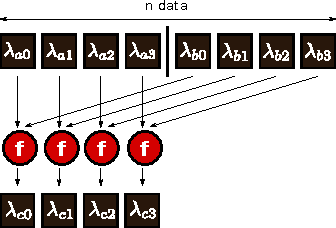
\includegraphics[scale=0.625]{figs/intra-simd}
        %\caption{Intra frame SIMD strategy}
        \label{fig:intra-simd}
      \end{figure}
    \end{column}
    \begin{column}[T]{6.0cm}
      \underline{Inter-frame SIMD strategy:}
      \begin{figure}[htp]
        \centering
        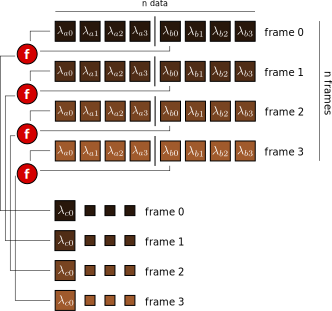
\includegraphics[scale=0.625]{figs/inter-simd}
        %\caption{Inter frame SIMD strategy}
        \label{fig:inter-simd}
      \end{figure}
    \end{column}
  \end{columns}
\end{frame}

% \begin{frame}{Polar Decoder: SC SIMDization Strategies}
%  \begin{columns}[t]
%    \begin{column}[T]{6.0cm}
%      Intra frame SIMD strategy:\\
%      ~~~$+$ low latency\\
%      ~~~$-$ leafs can't be vectorized
%    \end{column}
%    \begin{column}[T]{6.0cm}
%      Inter frame SIMD strategy:\\
%      ~~~$+$ high throughput\\
%      ~~~$-$ high latency
%    \end{column}
%  \end{columns}
% \end{frame}

\begin{frame}[containsverbatim,fragile]{Polar Application Programming Interface (Polar API)}
  \vspace{-0.2cm}
  \begin{itemize}
    \item Polar functions like $f$, $g$ and $h$ are implemented with \MIPP
    \item Efficient implementation compatible with NEON, SSE, AVX and AVX-512
    \item Mostly independent from the vectorization strategy (intra-/inter-frame)
  \end{itemize}
  \begin{minted}[linenos]{cpp}
template <typename R>
mipp::<R> f(const mipp::<R> la, const mipp::<R> lb) {
  return mipp::copysign(mipp::min(mipp::abs(la), mipp::abs(lb)),
                        mipp::sign(la, lb));
} // f(la, lb) = sign(la.lb).min(|la|, |lb|)

template <typename B, typename R>
mipp::<R> g(const mipp::<R> la, const mipp::<R> lb, const mipp::<B> s) {
  return mipp::copysign(la, s) + lb;
} // g(la, lb, sa) = (1-2s)la + lb

template <typename B>
mipp::<B> h(const mipp::<B> sa, const mipp::<B> sb) {
  return sa ^ sb;
} // h(sa, sb) = sa XOR sb
  \end{minted}
\end{frame}

\begin{frame}{SC Dynamic Versus Generated Implementation}
  \vspace{-0.4cm}
  \begin{columns}[t]
    \begin{column}[T]{6.0cm}
      \centering
      \scalebox{.65}{
      \setcounter{algocf}{0}
      \begin{algorithm}[H]
        \caption{Decoder SC Dynamic.}

        \SetKwProg{Fn}{Function}{}{}

        \Fn{$\DecoderSC()$}
        {
          \uIf{$\text{not a leaf}$}
          {
            $f()$ \Comment*[r]{multiple elements}

            $\DecoderSC()$ \Comment*[r]{left call}

            $g()$ \Comment*[r]{multiple elements}

            $\DecoderSC()$ \Comment*[r]{right call}

            $h()$ \Comment*[r]{multiple elements}
          }
          \Else(\Comment*[f]{a leaf node})
          {
            $\hardDecide() \text{~or \underline{frozen bit}}~;$
          }
        }
      \end{algorithm}
      }

      \only<1-2>{
      \begin{figure}[!h]
      \centering
      \begin{tikzpicture}[scale=0.65, every node/.style={transform shape}]
        % \path[use as bounding box] (-0.5,5.25) rectangle (14.0,-0.5);

        \tikzset{ any/.style ={draw=gray,     circle, minimum height=0.6cm, text=black, fill=gray!40                                                                              } }
        \tikzset{ frzn/.style={draw=black,    circle, minimum height=0.6cm, text=black                                                                                            } }
        \tikzset{ info/.style={draw=black,    circle, minimum height=0.6cm, text=white, fill=black                                                                                } }
        \tikzset{ r0/.style  ={draw=Paired-1, circle, minimum height=0.6cm, text=black, preaction={fill=Paired-1!40}, pattern=north west lines, pattern color=black!80!Paired-1!70} }
        \tikzset{ r1/.style  ={draw=Paired-3, circle, minimum height=0.6cm, text=black, preaction={fill=Paired-3!40}, pattern=north east lines, pattern color=black!80!Paired-3!70} }
        \tikzset{ rep/.style ={draw=Paired-7, circle, minimum height=0.6cm, text=black, preaction={fill=Paired-7!40}, pattern=crosshatch dots,  pattern color=black!80!Paired-7!70} }
        \tikzset{ spc4/.style={draw=Paired-5, circle, minimum height=0.6cm, text=black, preaction={fill=Paired-5!40}, pattern=horizontal lines, pattern color=black!80!Paired-5!70} }
        \tikzset{ spc/.style ={draw=Paired-9, circle, minimum height=0.6cm, text=black, preaction={fill=Paired-9!40}, pattern=grid,             pattern color=black!80!Paired-9!70} }

        \tikzset{ f/.style ={draw=black, text=black} }
        \tikzset{ g/.style ={draw=black, text=black} }
        \tikzset{ h/.style ={draw=black, text=black} }

        \only<1>{
        \node[frzn] (l3_g0) at (0.0, 0.0) {};
        \node[frzn] (l3_g1) at (1.0, 0.0) {};
        \node[frzn] (l3_g2) at (2.0, 0.0) {};
        \node[info] (l3_g3) at (3.0, 0.0) {};
        \node[frzn] (l3_g4) at (4.0, 0.0) {};
        \node[info] (l3_g5) at (5.0, 0.0) {};
        \node[info] (l3_g6) at (6.0, 0.0) {};
        \node[info] (l3_g7) at (7.0, 0.0) {};
        \node[any ] (l2_g0) at (0.5, 1.5) {};
        \node[any ] (l2_g1) at (2.5, 1.5) {};
        \node[any ] (l2_g2) at (4.5, 1.5) {};
        \node[any ] (l2_g3) at (6.5, 1.5) {};
        \node[any ] (l1_g0) at (1.5, 3.0) {};
        \node[any ] (l1_g1) at (5.5, 3.0) {};
        \node[any ] (l0_g0) at (3.5, 4.5) {};
        }

        \only<2->{
        \node[frzn] (l3_g0) at (0.0, 0.0) {\small{4}};
        \node[frzn] (l3_g1) at (1.0, 0.0) {\small{5}};
        \node[frzn] (l3_g2) at (2.0, 0.0) {\small{7}};
        \node[info] (l3_g3) at (3.0, 0.0) {\small{8}};
        \node[frzn] (l3_g4) at (4.0, 0.0) {};
        \node[info] (l3_g5) at (5.0, 0.0) {};
        \node[info] (l3_g6) at (6.0, 0.0) {};
        \node[info] (l3_g7) at (7.0, 0.0) {};
        \node[any ] (l2_g0) at (0.5, 1.5) {\small{3}};
        \node[any ] (l2_g1) at (2.5, 1.5) {\small{6}};
        \node[any ] (l2_g2) at (4.5, 1.5) {};
        \node[any ] (l2_g3) at (6.5, 1.5) {};
        \node[any ] (l1_g0) at (1.5, 3.0) {\small{2}};
        \node[any ] (l1_g1) at (5.5, 3.0) {\small{9}};
        \node[any ] (l0_g0) at (3.5, 4.5) {\small{1}};
        }

        \draw[f,->,>=latex] (l2_g0) -- (l3_g0) node [midway, above, text=black, xshift=-0.1cm, yshift=-0.1cm] {$f$};
        \draw[g,->,>=latex] (l2_g0) -- (l3_g1) node [midway, above, text=black, xshift=+0.1cm, yshift=-0.1cm] {$g$};
        \draw[h,->,>=latex] (l2_g0) to [out=180,in=120,looseness=8] (l2_g0) node [right, text=black, xshift=-1.25cm, yshift=0.4cm] {$h$};
        \draw[f,->,>=latex] (l2_g1) -- (l3_g2) node [midway, above, text=black, xshift=-0.1cm, yshift=-0.1cm] {$f$};
        \draw[g,->,>=latex] (l2_g1) -- (l3_g3) node [midway, above, text=black, xshift=+0.1cm, yshift=-0.1cm] {$g$};
        \draw[h,->,>=latex] (l2_g1) to [out=  0,in= 60,looseness=8] (l2_g1) node [right, text=black, xshift= 0.75cm, yshift=0.4cm] {$h$};
        \draw[f,->,>=latex] (l2_g2) -- (l3_g4) node [midway, above, text=black, xshift=-0.1cm, yshift=-0.1cm] {$f$};
        \draw[g,->,>=latex] (l2_g2) -- (l3_g5) node [midway, above, text=black, xshift=+0.1cm, yshift=-0.1cm] {$g$};
        \draw[h,->,>=latex] (l2_g2) to [out=180,in=120,looseness=8] (l2_g2) node [right, text=black, xshift=-1.25cm, yshift=0.4cm] {$h$};
        \draw[f,->,>=latex] (l2_g3) -- (l3_g6) node [midway, above, text=black, xshift=-0.1cm, yshift=-0.1cm] {$f$};
        \draw[g,->,>=latex] (l2_g3) -- (l3_g7) node [midway, above, text=black, xshift=+0.1cm, yshift=-0.1cm] {$g$};
        \draw[h,->,>=latex] (l2_g3) to [out=  0,in= 60,looseness=8] (l2_g3) node [right, text=black, xshift= 0.75cm, yshift=0.4cm] {$h$};
        \draw[f,->,>=latex] (l1_g0) -- (l2_g0) node [midway, above, text=black] {$f$};
        \draw[g,->,>=latex] (l1_g0) -- (l2_g1) node [midway, above, text=black] {$g$};
        \draw[h,->,>=latex] (l1_g0) to [out=180,in=120,looseness=8] (l1_g0) node [right, text=black, xshift=-1.25cm, yshift=0.4cm] {$h$};
        \draw[f,->,>=latex] (l1_g1) -- (l2_g2) node [midway, above, text=black] {$f$};
        \draw[g,->,>=latex] (l1_g1) -- (l2_g3) node [midway, above, text=black] {$g$};
        \draw[h,->,>=latex] (l1_g1) to [out=  0,in= 60,looseness=8] (l1_g1) node [right, text=black, xshift= 0.75cm, yshift=0.4cm] {$h$};
        \draw[f,->,>=latex] (l0_g0) -- (l1_g0) node [midway, above, text=black] {$f$};
        \draw[g,->,>=latex] (l0_g0) -- (l1_g1) node [midway, above, text=black] {$g$};
        \draw[h,->,>=latex] (l0_g0) to [out=0,in=60,looseness=8] (l0_g0) node [right, text=black, xshift=0.75cm, yshift=0.4cm] {$h$};
      \end{tikzpicture}
      \end{figure}
      }
    \end{column}
    \begin{column}[T]{6.0cm}
      \pause
      \centering
      \scalebox{.65}{
      \setcounter{algocf}{1}
      \begin{algorithm}[H]
        \caption{Decoder SC Generated.}

        \SetKwProg{Fn}{Function}{}{}

        \Fn{$\DecoderSC()$}
        {
          $f()$ \Comment*[r]{1 -> 2 [4 elmts]}

          $f()$ \Comment*[r]{2 -> 3 [2 elmts]}

          $f()$ \Comment*[r]{3 -> 4 [1 elmts]}

          $g()$ \Comment*[r]{3 -> 5 [1 elmts]}

          $h()$ \Comment*[r]{(4, 5) -> 3 [2 elmts]}

          $g()$ \Comment*[r]{2 -> 6 [2 elmts]}

          $f()$ \Comment*[r]{6 -> 7 [1 elmts]}

          $g()$ \Comment*[r]{6 -> 8 [1 elmts]}

          $\hardDecide()$ \Comment*[r]{8 -> 8 [1 elmts]}

          $h()$ \Comment*[r]{(7, 8) -> 6 [2 elmts]}

          $h()$ \Comment*[r]{(3, 6) -> 2 [4 elmts]}

          $g()$ \Comment*[r]{1 -> 9 [4 elmts]}

          $...$
        }
      \end{algorithm}
      }
    \end{column}
  \end{columns}

  \only<3->{
  \vspace{0.3cm}
  \begin{columns}
    \begin{column}[T]{6.0cm}
      \begin{itemize}
        \item High flexibility, same code can:
        \begin{itemize}
          \item Adapt to many code rate $R = K/N$
          \item Adapt to many frozen bits configurations
        \end{itemize}
        \item Overhead because of recursive calls
      \end{itemize}
    \end{column}
    \begin{column}[T]{6.0cm}
      \only<4->{
      \begin{itemize}
        \item Reduced flexibility, the code is generated for:
        \begin{itemize}
          \item Fixed code rate $R = K/N$
          \item Fixed frozen bits positions
        \end{itemize}
        \item No recursive call overhead: Higher throughput and lower latency
      \end{itemize}
      }
    \end{column}
  \end{columns}
  }
\end{frame}

\subsection[Source Code Generation]{Source Code Generation}

\begin{frame}{Issue}
  \begin{figure}[!h]
    \centering
    \scalebox{.5}{
    \begin{tikzpicture}%[scale=0.50, every node/.style={transform shape}]
    \begin{axis}[/pgfplots/table/ignore chars={ }, %footnotesize,
                 width=1.0\linewidth, height=0.7\linewidth,
                 ymode = log,
                 log basis y={2},
                 xticklabel style={black!70}, yticklabel style={black!70},
                 xlabel=Codeword size ($N$), ylabel=Decoder binary size (KB), grid=both, grid style={gray!30},
                 xmin=6, xmax=16,
                 xticklabels={$2^5$, $2^6$, $2^7$, $2^8$, $2^9$, $2^{10}$, $2^{11}$, $2^{12}$, $2^{13}$, $2^{14}$, $2^{15}$, $2^{16}$},
                 % yticklabels={2,4,8,16,32,64,128,256,512,1024,2048,4096},
                 yticklabels={2,8,32,128,512,2048},
                 grid style={dashed, gray!30},
                 %ymin=-5, ymax=102,
                 % tick align=outside, tickpos=left,
                 %label style={font=\large},
                 % tick label style={font=\large},
                 legend pos=south east, legend columns=1]
        \addplot[mark=square,   Paired-5,    semithick                              ] table [x index=0, y index=1] {../main/chapter4/fig/polar/sc_gen_l1i_size/dat/samples_generated_decoders_sizes.dat}; \label{plot:line1}
        \addplot[mark=triangle, Paired-1,    semithick                              ] table [x index=0, y index=3] {../main/chapter4/fig/polar/sc_gen_l1i_size/dat/samples_generated_decoders_sizes.dat}; \label{plot:line2}
        \addplot[mark=o,        Paired-1,    semithick, dashed, mark options={solid}] table [x index=0, y index=5] {../main/chapter4/fig/polar/sc_gen_l1i_size/dat/samples_generated_decoders_sizes.dat}; \label{plot:line3}
        \addplot[mark=none,     Paired-7,               dashed                      ] coordinates {(6,32) (16,32)}; \label{plot:line4}
    \end{axis}

    \matrix [draw,
             matrix of nodes,
             anchor=north,
             inner sep=2.3pt,
             fill=white,
             ampersand replacement=\&] at (2.3,6.5)
    {
        \ref{plot:line2} \& 32-bit \& intra-frame \\
        \ref{plot:line3} \& ~8-bit \& intra-frame \\
        \ref{plot:line1} \& 32-bit \& inter-frame \\
        \ref{plot:line4} \&        \& L1I size    \\
    };
  \end{tikzpicture}
  }
  \end{figure}
  \begin{itemize}
    \item \underline{Problem:} Codewords$~> N = 2^8$ exceeds the CPU instruction cache size
    \pause
    \vspace{0.2cm}
    \item \underline{Solution 1:} Do not store the memory addresses offsets in the generated code
    \pause
    \vspace{0.2cm}
    \item \underline{Solution 2:} Implement a sub-tree folding algorithm to reduce the binary size
  \end{itemize}
\end{frame}

\begin{frame}{Sub-tree Folding Algorithm}
  \begin{figure}[!h]
    \centering
    \scalebox{.4}{
    \begin{tikzpicture}[baseline]
      \tikzset{ any/.style ={draw=gray,     circle, minimum height=0.6cm, text=black, fill=gray!40                                                                              } }
      \tikzset{ frzn/.style={draw=black,    circle, minimum height=0.6cm, text=black                                                                                            } }
      \tikzset{ info/.style={draw=black,    circle, minimum height=0.6cm, text=black, fill=black                                                                                } }
      \tikzset{ r0/.style  ={draw=Paired-1, circle, minimum height=0.6cm, text=black, preaction={fill=Paired-1!40}, pattern=north west lines, pattern color=black!80!Paired-1!70} }
      \tikzset{ r1/.style  ={draw=Paired-3, circle, minimum height=0.6cm, text=black, preaction={fill=Paired-3!40}, pattern=north east lines, pattern color=black!80!Paired-3!70} }
      \tikzset{ rep/.style ={draw=Paired-7, circle, minimum height=0.6cm, text=black, preaction={fill=Paired-7!40}, pattern=crosshatch dots,  pattern color=black!80!Paired-7!70} }
      \tikzset{ spc4/.style={draw=Paired-5, circle, minimum height=0.6cm, text=black, preaction={fill=Paired-5!40}, pattern=horizontal lines, pattern color=black!80!Paired-5!70} }
      \tikzset{ spc/.style ={draw=Paired-9, circle, minimum height=0.6cm, text=black, preaction={fill=Paired-9!40}, pattern=grid,             pattern color=black!80!Paired-9!70} }

      \path[use as bounding box] (-0.5, +1.25) rectangle (14.5, -1.3);

      \node[any,  label={[black,align=center]above:\small{Any}}                              ] (any)  at ( 0.0, 0.0) {};
      \node[frzn, label={[black,align=center]above:\small{Frozen bit}\\\small{(leaf)}}       ] (frz)  at ( 2.0, 0.0) {};
      \node[info, label={[black,align=center]above:\small{Info. bit}\\\small{(leaf)}}        ] (ufrz) at ( 4.0, 0.0) {};
      \node[r0,   label={[black,align=center]above:\small{\texttt{R0}}}                      ] (r0)   at ( 6.0, 0.0) {};
      \node[r1,   label={[black,align=center]above:\small{\texttt{R1}}}                      ] (r1)   at ( 8.0, 0.0) {};
      \node[rep,  label={[black,align=center]above:\small{\texttt{REP}}}                     ] (rep)  at (10.0, 0.0) {};
      \node[spc4, label={[black,align=center]above:\small{\texttt{SPC}$_\text{\texttt{4}}$}} ] (spc4) at (12.0, 0.0) {};
      \node[spc,  label={[black,align=center]above:\small{\texttt{SPC}$_\text{\texttt{4+}}$}}] (spc)  at (14.0, 0.0) {};

      \draw[<-,>=latex        ] (2.5, -1.25) -- ( 5.5, -1.25) node [midway, above, text=black] {\small{Left edge ($f$)}};
      \draw[->,>=latex, dashed] (8.5, -1.25) -- (11.5, -1.25) node [midway, above, text=black] {\small{Right edge ($g$)}};
    \end{tikzpicture}
    }
  \end{figure}

  \begin{columns}
  \begin{column}[T]{5.0cm}
  \begin{figure}[!h]
    \centering
    \scalebox{.4}{
    \begin{tikzpicture}[baseline]
      \tikzset{ any/.style ={draw=gray,     circle, minimum height=0.6cm, text=black, fill=gray!40                                                                              } }
      \tikzset{ frzn/.style={draw=black,    circle, minimum height=0.6cm, text=black                                                                                            } }
      \tikzset{ info/.style={draw=black,    circle, minimum height=0.6cm, text=black, fill=black                                                                                } }
      \tikzset{ r0/.style  ={draw=Paired-1, circle, minimum height=0.6cm, text=black, preaction={fill=Paired-1!40}, pattern=north west lines, pattern color=black!80!Paired-1!70} }
      \tikzset{ r1/.style  ={draw=Paired-3, circle, minimum height=0.6cm, text=black, preaction={fill=Paired-3!40}, pattern=north east lines, pattern color=black!80!Paired-3!70} }
      \tikzset{ rep/.style ={draw=Paired-7, circle, minimum height=0.6cm, text=black, preaction={fill=Paired-7!40}, pattern=crosshatch dots,  pattern color=black!80!Paired-7!70} }
      \tikzset{ spc4/.style={draw=Paired-5, circle, minimum height=0.6cm, text=black, preaction={fill=Paired-5!40}, pattern=horizontal lines, pattern color=black!80!Paired-5!70} }
      \tikzset{ spc/.style ={draw=Paired-9, circle, minimum height=0.6cm, text=black, preaction={fill=Paired-9!40}, pattern=grid,             pattern color=black!80!Paired-9!70} }

      \node[any] (l0_n0)  at ( 6.5, 6.0) {};

      \node[any] (l1_n0)  at ( 4.5, 5.0) {};
      \node[any] (l1_n1)  at ( 8.5, 5.0) {};

      \draw[->,>=latex        ] (l0_n0) -- (l1_n0);
      \draw[->,>=latex, dashed] (l0_n0) -- (l1_n1);

      \node[any] (l2_n0)  at ( 1.5, 4.0) {};
      \node[any] (l2_n1)  at ( 4.5, 4.0) {};
      \node[any] (l2_n2)  at ( 8.5, 4.0) {};
      \node[any] (l2_n3)  at (11.5, 4.0) {};

      \draw[->,>=latex        ] (l1_n0) -- (l2_n0);
      \draw[->,>=latex, dashed] (l1_n0) -- (l2_n1);
      \draw[->,>=latex        ] (l1_n1) -- (l2_n2);
      \draw[->,>=latex, dashed] (l1_n1) -- (l2_n3);

      \node[r0 ] (l3_n0)  at ( 0.5, 3.0) {};
      \node[any] (l3_n1)  at ( 1.5, 3.0) {};
      \node[any] (l3_n2)  at ( 4.0, 3.0) {};
      \node[any] (l3_n3)  at ( 5.0, 3.0) {};
      \node[any] (l3_n4)  at ( 8.0, 3.0) {};
      \node[any] (l3_n5)  at ( 9.0, 3.0) {};
      \node[any] (l3_n6)  at (11.5, 3.0) {};
      \node[r1 ] (l3_n7)  at (12.5, 3.0) {};

      \draw[->,>=latex        ] (l2_n0) -- (l3_n0);
      \draw[->,>=latex, dashed] (l2_n0) -- (l3_n1);
      \draw[->,>=latex        ] (l2_n1) -- (l3_n2);
      \draw[->,>=latex, dashed] (l2_n1) -- (l3_n3);
      \draw[->,>=latex        ] (l2_n2) -- (l3_n4);
      \draw[->,>=latex, dashed] (l2_n2) -- (l3_n5);
      \draw[->,>=latex        ] (l2_n3) -- (l3_n6);
      \draw[->,>=latex, dashed] (l2_n3) -- (l3_n7);

      \node[r0 ] (l4_n0)  at ( 0.5, 2.0) {};
      \node[any] (l4_n1)  at ( 1.5, 2.0) {};
      \node[r0 ] (l4_n2)  at ( 3.0, 2.0) {};
      \node[any] (l4_n3)  at ( 4.0, 2.0) {};
      \node[any] (l4_n4)  at ( 5.0, 2.0) {};
      \node[spc] (l4_n5)  at ( 6.0, 2.0) {};
      \node[rep] (l4_n6)  at ( 7.0, 2.0) {};
      \node[any] (l4_n7)  at ( 8.0, 2.0) {};
      \node[any] (l4_n8)  at ( 9.0, 2.0) {};
      \node[r1 ] (l4_n9)  at (10.0, 2.0) {};
      \node[any] (l4_n10) at (11.5, 2.0) {};
      \node[r1 ] (l4_n11) at (12.5, 2.0) {};

      \draw[->,>=latex        ] (l3_n1) -- (l4_n0);
      \draw[->,>=latex, dashed] (l3_n1) -- (l4_n1);
      \draw[->,>=latex        ] (l3_n2) -- (l4_n2);
      \draw[->,>=latex, dashed] (l3_n2) -- (l4_n3);
      \draw[->,>=latex        ] (l3_n3) -- (l4_n4);
      \draw[->,>=latex, dashed] (l3_n3) -- (l4_n5);
      \draw[->,>=latex        ] (l3_n4) -- (l4_n6);
      \draw[->,>=latex, dashed] (l3_n4) -- (l4_n7);
      \draw[->,>=latex        ] (l3_n5) -- (l4_n8);
      \draw[->,>=latex, dashed] (l3_n5) -- (l4_n9);
      \draw[->,>=latex        ] (l3_n6) -- (l4_n10);
      \draw[->,>=latex, dashed] (l3_n6) -- (l4_n11);

      \node[r0  ] (l5_n0)  at ( 0.5, 1.0) {};
      \node[any ] (l5_n1)  at ( 1.5, 1.0) {};
      \node[rep ] (l5_n2)  at ( 3.0, 1.0) {};
      \node[spc4] (l5_n3)  at ( 4.0, 1.0) {};
      \node[rep ] (l5_n4)  at ( 5.0, 1.0) {};
      \node[spc4] (l5_n5)  at ( 6.0, 1.0) {};
      \node[rep ] (l5_n6)  at ( 7.0, 1.0) {};
      \node[spc4] (l5_n7)  at ( 8.0, 1.0) {};
      \node[rep ] (l5_n8)  at ( 9.0, 1.0) {};
      \node[spc4] (l5_n9)  at (10.0, 1.0) {};
      \node[any ] (l5_n10) at (11.5, 1.0) {};
      \node[r1  ] (l5_n11) at (12.5, 1.0) {};

      \draw[->,>=latex        ] (l4_n1)  -- (l5_n0);
      \draw[->,>=latex, dashed] (l4_n1)  -- (l5_n1);
      \draw[->,>=latex        ] (l4_n3)  -- (l5_n2);
      \draw[->,>=latex, dashed] (l4_n3)  -- (l5_n3);
      \draw[->,>=latex        ] (l4_n4)  -- (l5_n4);
      \draw[->,>=latex, dashed] (l4_n4)  -- (l5_n5);
      \draw[->,>=latex        ] (l4_n7)  -- (l5_n6);
      \draw[->,>=latex, dashed] (l4_n7)  -- (l5_n7);
      \draw[->,>=latex        ] (l4_n8)  -- (l5_n8);
      \draw[->,>=latex, dashed] (l4_n8)  -- (l5_n9);
      \draw[->,>=latex        ] (l4_n10) -- (l5_n10);
      \draw[->,>=latex, dashed] (l4_n10) -- (l5_n11);

      \node[r0] (l6_n0) at ( 1.0, 0.0) {};
      \node[r1] (l6_n1) at ( 2.0, 0.0) {};
      \node[r0] (l6_n2) at (11.0, 0.0) {};
      \node[r1] (l6_n3) at (12.0, 0.0) {};

      \draw[->,>=latex        ] (l5_n1)  -- (l6_n0);
      \draw[->,>=latex, dashed] (l5_n1)  -- (l6_n1);
      \draw[->,>=latex        ] (l5_n10) -- (l6_n2);
      \draw[->,>=latex, dashed] (l5_n10) -- (l6_n3);

      \node[draw=Paired-5, rounded corners=2pt, dashed, fit=(l5_n1) (l6_n0) (l6_n1)] {};
      \node[draw=Paired-5, rounded corners=2pt, dashed, fit=(l5_n10) (l6_n2) (l6_n3)] {};

      \node[draw=Paired-3, rounded corners=2pt, dashed, fit=(l4_n3) (l5_n2) (l5_n3)] {};
      \node[draw=Paired-3, rounded corners=2pt, dashed, fit=(l4_n4) (l5_n4) (l5_n5)] {};
      \node[draw=Paired-3, rounded corners=2pt, dashed, fit=(l4_n7) (l5_n6) (l5_n7)] {};
      \node[draw=Paired-3, rounded corners=2pt, dashed, fit=(l4_n8) (l5_n8) (l5_n9)] {};
    \end{tikzpicture}
    }
  \end{figure}
  \end{column}
  \begin{column}[T]{1.0cm}
    \vspace{2cm}
    \centering
    {\color{black}\Large\MVRightarrow}
  \end{column}
  \begin{column}[T]{5.0cm}
    \begin{figure}[!h]
    \centering
    \scalebox{.4}{
    \begin{tikzpicture}[baseline]
      \tikzset{ any/.style ={draw=gray,     circle, minimum height=0.6cm, text=black, fill=gray!40                                                                              } }
      \tikzset{ frzn/.style={draw=black,    circle, minimum height=0.6cm, text=black                                                                                            } }
      \tikzset{ info/.style={draw=black,    circle, minimum height=0.6cm, text=black, fill=black                                                                                } }
      \tikzset{ r0/.style  ={draw=Paired-1, circle, minimum height=0.6cm, text=black, preaction={fill=Paired-1!40}, pattern=north west lines, pattern color=black!80!Paired-1!70} }
      \tikzset{ r1/.style  ={draw=Paired-3, circle, minimum height=0.6cm, text=black, preaction={fill=Paired-3!40}, pattern=north east lines, pattern color=black!80!Paired-3!70} }
      \tikzset{ rep/.style ={draw=Paired-7, circle, minimum height=0.6cm, text=black, preaction={fill=Paired-7!40}, pattern=crosshatch dots,  pattern color=black!80!Paired-7!70} }
      \tikzset{ spc4/.style={draw=Paired-5, circle, minimum height=0.6cm, text=black, preaction={fill=Paired-5!40}, pattern=horizontal lines, pattern color=black!80!Paired-5!70} }
      \tikzset{ spc/.style ={draw=Paired-9, circle, minimum height=0.6cm, text=black, preaction={fill=Paired-9!40}, pattern=grid,             pattern color=black!80!Paired-9!70} }

      \node[any] (l0_n0)  at ( 6.5, 6.0) {};

      \node[any] (l1_n0)  at ( 4.5, 5.0) {};
      \node[any] (l1_n1)  at ( 8.5, 5.0) {};

      \draw[->,>=latex        ] (l0_n0) -- (l1_n0);
      \draw[->,>=latex, dashed] (l0_n0) -- (l1_n1);

      \node[any] (l2_n0)  at ( 1.5, 4.0) {};
      \node[any] (l2_n1)  at ( 4.5, 4.0) {};
      \node[any] (l2_n2)  at ( 8.5, 4.0) {};
      \node[any] (l2_n3)  at (11.5, 4.0) {};

      \draw[->,>=latex        ] (l1_n0) -- (l2_n0);
      \draw[->,>=latex, dashed] (l1_n0) -- (l2_n1);
      \draw[->,>=latex        ] (l1_n1) -- (l2_n2);
      \draw[->,>=latex, dashed] (l1_n1) -- (l2_n3);

      \node[r0 ] (l3_n0)  at ( 0.5, 3.0) {};
      \node[any] (l3_n1)  at ( 1.5, 3.0) {};
      \node[any] (l3_n2)  at ( 4.0, 3.0) {};
      \node[any] (l3_n3)  at ( 5.0, 3.0) {};
      \node[any] (l3_n4)  at ( 8.0, 3.0) {};
      \node[any] (l3_n5)  at ( 9.0, 3.0) {};
      \node[any] (l3_n6)  at (11.5, 3.0) {};
      \node[r1 ] (l3_n7)  at (12.5, 3.0) {};

      \draw[->,>=latex        ] (l2_n0) -- (l3_n0);
      \draw[->,>=latex, dashed] (l2_n0) -- (l3_n1);
      \draw[->,>=latex        ] (l2_n1) -- (l3_n2);
      \draw[->,>=latex, dashed] (l2_n1) -- (l3_n3);
      \draw[->,>=latex        ] (l2_n2) -- (l3_n4);
      \draw[->,>=latex, dashed] (l2_n2) -- (l3_n5);
      \draw[->,>=latex        ] (l2_n3) -- (l3_n6);
      \draw[->,>=latex, dashed] (l2_n3) -- (l3_n7);

      \node[any] (l4_n0) at ( 1.50, 2.0) {};
      \node[r0 ] (l4_n1) at ( 2.75, 2.0) {};
      \node[spc] (l4_n2) at ( 5.00, 2.0) {};
      \node[any] (l4_n3) at ( 6.50, 2.0) {};
      \node[rep] (l4_n4) at ( 8.00, 2.0) {};
      \node[r1 ] (l4_n5) at (10.25, 2.0) {};
      \node[any] (l4_n6) at (11.50, 2.0) {};

      \draw[->,>=latex, dashed] (l3_n1) -- (l4_n0);
      \draw[->,>=latex        ] (l3_n1) -- (l4_n1);
      \draw[->,>=latex        ] (l3_n2) -- (l4_n1);
      \draw[->,>=latex, dashed] (l3_n2) -- (l4_n3);
      \draw[->,>=latex, dashed] (l3_n3) -- (l4_n2);
      \draw[->,>=latex        ] (l3_n3) -- (l4_n3);
      \draw[->,>=latex, dashed] (l3_n4) -- (l4_n3);
      \draw[->,>=latex        ] (l3_n4) -- (l4_n4);
      \draw[->,>=latex        ] (l3_n5) -- (l4_n3);
      \draw[->,>=latex, dashed] (l3_n5) -- (l4_n5);
      \draw[->,>=latex, dashed] (l3_n6) -- (l4_n5);
      \draw[->,>=latex        ] (l3_n6) -- (l4_n6);

      \node[r0  ] (l5_n0)  at ( 0.50, 1.0) {};
      \node[any ] (l5_n1)  at ( 1.50, 1.0) {};
      \node[rep ] (l5_n2)  at ( 6.00, 1.0) {};
      \node[spc4] (l5_n3)  at ( 7.00, 1.0) {};
      \node[r1  ] (l5_n4)  at (12.50, 1.0) {};

      \draw[->,>=latex        ] (l4_n0) -- (l5_n0);
      \draw[->,>=latex, dashed] (l4_n0) -- (l5_n1);
      \draw[->,>=latex        ] (l4_n3) -- (l5_n2);
      \draw[->,>=latex, dashed] (l4_n3) -- (l5_n3);
      % \draw[->,>=latex        ] (l4_n6) -- (l5_n1);
      \draw[->,>=latex        ] (l4_n6) to[out=230,in=0] (l5_n1);
      \draw[->,>=latex, dashed] (l4_n6) -- (l5_n4);

      \node[r0] (l6_n0) at ( 1.0, 0.0) {};
      \node[r1] (l6_n1) at ( 2.0, 0.0) {};

      \draw[->,>=latex        ] (l5_n1) -- (l6_n0);
      \draw[->,>=latex, dashed] (l5_n1) -- (l6_n1);

      \node[draw=Paired-5, rounded corners=2pt, dashed, fit=(l5_n1) (l6_n0) (l6_n1)] {};
      \node[draw=Paired-3, rounded corners=2pt, dashed, fit=(l4_n3) (l5_n2) (l5_n3)] {};
    \end{tikzpicture}
    }
  \end{figure}
  \end{column}
  \end{columns}
  \vfill
  \begin{itemize}
    \item Find similar sub-patterns and create functions for them
    \item Compromise between the number of functions calls and the binary size
    \item Threshold to avoid functions that contain a too small number of Polar functions
  \end{itemize}
\end{frame}

\begin{frame}{Results}
  \vspace{-0.5cm}
  \begin{columns}
  \begin{column}[T]{6.0cm}
    \begin{figure}[!h]
      \centering
      \scalebox{.5}{
      \begin{tikzpicture}%[scale=0.50, every node/.style={transform shape}]
      \begin{axis}[/pgfplots/table/ignore chars={ }, %footnotesize,
                   width=2.0\linewidth, height=1.4\linewidth,
                   ymode = log,
                   log basis y={2},
                   xticklabel style={black!70}, yticklabel style={black!70},
                   xlabel=Codeword size ($N$), ylabel=Decoder binary size (KB), grid=both, grid style={gray!30},
                   xmin=6, xmax=16,
                   xticklabels={$2^5$, $2^6$, $2^7$, $2^8$, $2^9$, $2^{10}$, $2^{11}$, $2^{12}$, $2^{13}$, $2^{14}$, $2^{15}$, $2^{16}$},
                   % yticklabels={2,4,8,16,32,64,128,256,512,1024,2048,4096},
                   yticklabels={2,8,32,128,512,2048},
                   grid style={dashed, gray!30},
                   %ymin=-5, ymax=102,
                   % tick align=outside, tickpos=left,
                   %label style={font=\large},
                   % tick label style={font=\large},
                   legend pos=south east, legend columns=1]
          \addplot[mark=square,   Paired-5,    semithick                              ] table [x index=0, y index=1] {../main/chapter4/fig/polar/sc_gen_l1i_size/dat/samples_generated_decoders_sizes.dat}; \label{plot:line1}
          \addplot[mark=triangle, Paired-1,    semithick                              ] table [x index=0, y index=3] {../main/chapter4/fig/polar/sc_gen_l1i_size/dat/samples_generated_decoders_sizes.dat}; \label{plot:line2}
          \addplot[mark=o,        Paired-1,    semithick, dashed, mark options={solid}] table [x index=0, y index=5] {../main/chapter4/fig/polar/sc_gen_l1i_size/dat/samples_generated_decoders_sizes.dat}; \label{plot:line3}
          \addplot[mark=none,     Paired-7,               dashed                      ] coordinates {(6,32) (16,32)}; \label{plot:line4}
      \end{axis}

      \matrix[draw,
              matrix of nodes,
              anchor=north,
              inner sep=2.3pt,
              fill=white,
              ampersand replacement=\&] at (2.3,6.5)
      {
          \ref{plot:line2} \& 32-bit \& intra-frame \\
          \ref{plot:line3} \& ~8-bit \& intra-frame \\
          \ref{plot:line1} \& 32-bit \& inter-frame \\
          \ref{plot:line4} \&        \& L1I size    \\
      };
    \end{tikzpicture}
    }
    \caption*{Without compression}
    \end{figure}
  \end{column}
  \begin{column}[T]{6.0cm}
    \begin{figure}[!h]
    \centering
    \scalebox{.5}{
    \begin{tikzpicture}
    \begin{axis}[/pgfplots/table/ignore chars={ }, %footnotesize,
                 width=2.0\linewidth, height=1.4\linewidth,
                 ymode = log,
                 log basis y={2},
                 xticklabel style={black!70}, yticklabel style={black!70},
                 xlabel=Codeword size ($N$), ylabel=Decoder binary size (KB), grid=both, grid style={gray!30},
                 xmin=6, xmax=16,
                 xticklabels={$2^5$, $2^6$, $2^7$, $2^8$, $2^9$, $2^{10}$, $2^{11}$, $2^{12}$, $2^{13}$, $2^{14}$, $2^{15}$, $2^{16}$},
                 yticklabels={0,1,2,4,8,16,32,64},
                 grid style={dashed, gray!30},
                 %ymin=-5, ymax=102,
                 % tick align=outside, tickpos=left,
                 %label style={font=\large},
                 % tick label style={font=\large},
                 legend pos=south east, legend columns=1]
        \addplot[mark=square,   Paired-5,    semithick                              ] table [x index=0, y index=1] {../main/chapter4/fig/polar/sc_gen_l1i_size/dat/samples_generated_decoders_sizes_after_compression.dat}; \label{plot:line1}
        \addplot[mark=triangle, Paired-1,    semithick                              ] table [x index=0, y index=3] {../main/chapter4/fig/polar/sc_gen_l1i_size/dat/samples_generated_decoders_sizes_after_compression.dat}; \label{plot:line2}
        \addplot[mark=o,        Paired-1,    semithick, dashed, mark options={solid}] table [x index=0, y index=5] {../main/chapter4/fig/polar/sc_gen_l1i_size/dat/samples_generated_decoders_sizes_after_compression.dat}; \label{plot:line3}
        \addplot[mark=none,     Paired-7,    dashed                                 ] coordinates {(6,32) (16,32)}; \label{plot:line4}

        \node[anchor=west] (source) at (axis cs:11.8,3.5){\textbullet\ Enable sub-tree folding};
        \draw[->,thick] (axis cs:12, 4) -- (axis cs:12, 6.5);
    \end{axis}
    \end{tikzpicture}
    }
    \caption*{With compression}
    \end{figure}
  \end{column}
  \end{columns}
  \vfill
  \begin{itemize}
    \item \underline{Problem:} Codewords$~> N = 2^8$ exceeds the CPU instruction cache size
    \vspace{0.2cm}
    \item \underline{Solution 1:} Do not store the memory addresses offsets in the generated code
    \vspace{0.2cm}
    \item \underline{Solution 2:} Implement a sub-tree folding algorithm to reduce the binary size
  \end{itemize}
\end{frame}

\subsection[Propositions]{Propositions}

\begin{frame}{Propositions}
  \vfill
  \underline{Propositions:}

  \vspace{0.3cm}
  \begin{enumerate}
    \item High performance implementation of the \textbf{dynamic SC scheduling}
    \begin{itemize}
      \item Support intra-/inter-frame SIMDization thanks to the Polar API
      \item Compatible with tree pruning techniques
      \item Fine tuned implementation with \textbf{template meta-programming techniques}
    \end{itemize}
    \pause
    \vspace{0.3cm}
    \item Polar ECC Decoder \textbf{Generation Environment} (P-EDGE)
    \begin{itemize}
      \item Support intra-/inter-frame SIMDization thanks to the Polar API
      \item Compatible with tree pruning techniques
      \item Source code generation environment for \textbf{highest possible performances}
    \end{itemize}
  \end{enumerate}
  \vfill
\end{frame}

% \begin{frame}{Polar Decoder: Successive Cancellation List Algorithm}
%   \begin{itemize}
%     \item Based on the Successive Cancellation decoder
%     \item Maintains a finite list of $L$ possible decoding trees
%     \item Chooses the most likely tree according to a metric
%     \item Decoding performance are better for short to medium size codewords
%     \item Can be combined with a CRC code to discriminate the metric
%       \\\vspace*{.5em}
%       {\color{bleuUni}\Large\MVRightarrow} Decoding performance is, again, improved
%   \end{itemize}
% \end{frame}

\subsection[Evaluations and Comparisons]{Evaluations and Comparisons}

\begin{frame}{Experimentation Protocol}

  \begin{table}[htp]
    \centering
    % \caption
    %   [Specification of the x86 platforms for the polar decoders experiments.]
    %   {Specification of the x86 platforms.}
    % \label{tab:eval_polar_sc_specs_x86}
    {\small\resizebox{1.0\linewidth}{!}{
    \begin{tabular}{c | c c c}
                                  & \textbf{E3-1225}        & \textbf{i7-2600}        & \textbf{i7-4850HQ}         \\
    \hline
    \hline
    \multirow{1}{*}{\textbf{CPU}} & Intel\R Xeon\TM E3-1225 & Intel\R Core\TM i7-2600 & Intel\R Core\TM  i7-4850HQ \\
    \textbf{Cores/Freq.}          & 4 cores, 3.1-3.4 Ghz    & 4 cores, 3.4-3.8 GHz    & 4 cores, 2.3-3.5 GHz       \\
    \textbf{Arch.}                & \emph{Sandy Bridge}     & \emph{Sandy Bridge}     & \emph{Crystal Well}        \\
    \textbf{Process}              & 32 nm                   & 32 nm                   & 22 nm                      \\
    \multirow{1}{*}{\textbf{LLC}} & L3 6 MB                 & L3 8 MB                 & L3 6 MB                    \\
    \end{tabular}
    }}
  \end{table}

  \begin{itemize}
    \item GCC flags and version
    \item Focus on the generated decoders (intra and inter)
  \end{itemize}

\end{frame}

\begin{frame}{Impact of the Tree Pruning}
  \begin{columns}
  \begin{column}[T]{6cm}
    \begin{figure}[!h]
    \centering
    \scalebox{.5}{
    \begin{tikzpicture}[every axis/.style={
                        /pgfplots/table/ignore chars={|}, %footnotesize,
                        width=2.0\linewidth, height=1.40\linewidth,
                        xticklabel style={black!70}, yticklabel style={black!70},
                        % tick align=outside, tickpos=left,
                        ybar stacked, bar width=14pt,
                        legend style={at={(0.39,0.95)}, anchor=north}, legend columns=-1,
                        ylabel={Coded throughput (Mb/s)}, xlabel={Code rate ($R = K / N$)},
                        ymajorgrids, grid style={gray!30}, grid style={dashed, gray!50}, xmin=0.05, xmax=0.45, xtick=data, ymin=0, ymax=550.0,
                        x tick label style={rotate=-45}, xticklabels={1/5, 1/2, 5/6, 9/10}}]

      \begin{axis}[]
        \addplot+[draw=black,    fill=black!50                                                                                 ] table [x=R, y expr=\thisrowno{4}              ] {../main/chapter2/fig/polar/sc_tree_cut/dat/E31225_samples_intra_32b_opti_spc4+.dat};
        \only<2->{
        \addplot+[draw=Paired-1, fill=Paired-1!40, postaction={pattern color = black!80!Paired-1!70, pattern=north west  lines}] table [x=R, y expr=\thisrowno{5}-\thisrowno{4}] {../main/chapter2/fig/polar/sc_tree_cut/dat/E31225_samples_intra_32b_opti_spc4+.dat};
        }
        \only<3->{
        \addplot+[draw=Paired-3, fill=Paired-3!40, postaction={pattern color = black!80!Paired-3!70, pattern=north east  lines}] table [x=R, y expr=\thisrowno{6}-\thisrowno{5}] {../main/chapter2/fig/polar/sc_tree_cut/dat/E31225_samples_intra_32b_opti_spc4+.dat};
        }
        \only<4->{
        \addplot+[draw=Paired-7, fill=Paired-7!40, postaction={pattern color = black!80!Paired-7!70, pattern=crosshatch  dots} ] table [x=R, y expr=\thisrowno{7}-\thisrowno{6}] {../main/chapter2/fig/polar/sc_tree_cut/dat/E31225_samples_intra_32b_opti_spc4+.dat};
        }
        \only<6->{
        \addplot+[draw=Paired-5, fill=Paired-5!40, postaction={pattern color = black!80!Paired-5!70, pattern=horizontal lines} ] table [x=R, y expr=\thisrowno{8}-\thisrowno{7}] {../main/chapter2/fig/polar/sc_tree_cut/dat/E31225_samples_intra_32b_opti_spc4+.dat};
        }
        \only<5->{
        \addplot+[draw=Paired-9, fill=Paired-9!40, postaction={pattern color = black!80!Paired-9!70, pattern=grid}             ] table [x=R, y expr=\thisrowno{9}-\thisrowno{8}] {../main/chapter2/fig/polar/sc_tree_cut/dat/E31225_samples_intra_32b_opti_spc4+.dat};
        }
        \only<1-5>{
        \legend{\texttt{ref}\text{ }, \texttt{R0}\text{ }, \texttt{R1}\text{ }, \texttt{REP}\text{ }, $\texttt{SPC}_\text{\texttt{4+}}$}
        }
        \only<6>{
        \legend{\texttt{ref}\text{ }, \texttt{R0}\text{ }, \texttt{R1}\text{ }, \texttt{REP}\text{ }, $\texttt{SPC}_\text{\texttt{4}}$\text{ } , $\texttt{SPC}_\text{\texttt{4+}}$}
        }
      \end{axis}

      \only<6->{
      \begin{axis}[bar shift=-20pt, hide axis]
        \addplot+[draw=black,    fill=black!50                                                                                 ] table [x=R, y expr=\thisrowno{4}              ] {../main/chapter2/fig/polar/sc_tree_cut/dat/E31225_samples_intra_32b_opti_spc4.dat};
        \addplot+[draw=Paired-1, fill=Paired-1!40, postaction={pattern color = black!80!Paired-1!70, pattern=north west  lines}] table [x=R, y expr=\thisrowno{5}-\thisrowno{4}] {../main/chapter2/fig/polar/sc_tree_cut/dat/E31225_samples_intra_32b_opti_spc4.dat};
        \addplot+[draw=Paired-3, fill=Paired-3!40, postaction={pattern color = black!80!Paired-3!70, pattern=north east  lines}] table [x=R, y expr=\thisrowno{6}-\thisrowno{5}] {../main/chapter2/fig/polar/sc_tree_cut/dat/E31225_samples_intra_32b_opti_spc4.dat};
        \addplot+[draw=Paired-7, fill=Paired-7!40, postaction={pattern color = black!80!Paired-7!70, pattern=crosshatch  dots} ] table [x=R, y expr=\thisrowno{7}-\thisrowno{6}] {../main/chapter2/fig/polar/sc_tree_cut/dat/E31225_samples_intra_32b_opti_spc4.dat};
        \addplot+[draw=Paired-5, fill=Paired-5!40, postaction={pattern color = black!80!Paired-5!70, pattern=horizontal lines} ] table [x=R, y expr=\thisrowno{8}-\thisrowno{7}] {../main/chapter2/fig/polar/sc_tree_cut/dat/E31225_samples_intra_32b_opti_spc4.dat};
      \end{axis}
      }

      \only<7->{
      \begin{axis}[bar shift=+20pt,hide axis]
        \addplot+[draw=black,    fill=black!50                                                                                 ] table [x=R, y expr=\thisrowno{4}               ] {../main/chapter2/fig/polar/sc_tree_cut/dat/E31225_samples_intra_32b_opti_spc16-.dat};
        \addplot+[draw=Paired-1, fill=Paired-1!40, postaction={pattern color = black!80!Paired-1!70, pattern=north west  lines}] table [x=R, y expr=\thisrowno{5}-\thisrowno{4} ] {../main/chapter2/fig/polar/sc_tree_cut/dat/E31225_samples_intra_32b_opti_spc16-.dat};
        \addplot+[draw=Paired-3, fill=Paired-3!40, postaction={pattern color = black!80!Paired-3!70, pattern=north east  lines}] table [x=R, y expr=\thisrowno{6}-\thisrowno{5} ] {../main/chapter2/fig/polar/sc_tree_cut/dat/E31225_samples_intra_32b_opti_spc16-.dat};
        \addplot+[draw=Paired-7, fill=Paired-7!40, postaction={pattern color = black!80!Paired-7!70, pattern=crosshatch  dots} ] table [x=R, y expr=\thisrowno{7}-\thisrowno{6} ] {../main/chapter2/fig/polar/sc_tree_cut/dat/E31225_samples_intra_32b_opti_spc16-.dat};
        \addplot+[draw=Paired-5, fill=Paired-5!40, postaction={pattern color = black!80!Paired-5!70, pattern=horizontal lines} ] table [x=R, y expr=\thisrowno{8}-\thisrowno{7} ] {../main/chapter2/fig/polar/sc_tree_cut/dat/E31225_samples_intra_32b_opti_spc16-.dat};
        \addplot+[draw=Paired-9, fill=Paired-9!40, postaction={pattern color = black!80!Paired-9!70, pattern=grid}             ] table [x=R, y expr=\thisrowno{9}-\thisrowno{8} ] {../main/chapter2/fig/polar/sc_tree_cut/dat/E31225_samples_intra_32b_opti_spc16-.dat};
        \addplot+[draw=Paired-9, fill=Paired-9!10, postaction={pattern color = black!80!Paired-9!70, pattern=grid}             ] table [x=R, y expr=\thisrowno{10}-\thisrowno{9}] {../main/chapter2/fig/polar/sc_tree_cut/dat/E31225_samples_intra_32b_opti_spc16-.dat};
        \legend{\texttt{ref}\text{ }, \texttt{R0}\text{ }, \texttt{R1}\text{ }, \texttt{REP}\text{ }, $\texttt{SPC}_\text{\texttt{4}}$\text{ } , $\texttt{SPC}_\text{\texttt{4+}}$ , $\texttt{SPC}_\text{\texttt{16-}}$}
      \end{axis}
      }
    \end{tikzpicture}
    }
    \end{figure}
  \end{column}
  \begin{column}[T]{6cm}
    \begin{figure}[!h]
    \centering
    \scalebox{.5}{
    \begin{tikzpicture}[every axis/.style={
                        /pgfplots/table/ignore chars={|}, %footnotesize,
                        width=2.0\linewidth, height=1.40\linewidth,
                        xticklabel style={black!70}, yticklabel style={black!70},
                        % tick align=outside, tickpos=left,
                        ybar stacked, bar width=14pt,
                        legend style={at={(0.39,0.95)}, anchor=north}, legend columns=-1,
                        ylabel={Coded throughput (Mb/s)}, xlabel={Code rate ($R = K / N$)},
                        ymajorgrids, grid style={gray!30}, grid style={dashed, gray!50}, xmin=0.05, xmax=0.45, xtick=data, ymin=0, ymax=1900.0,
                        x tick label style={rotate=-45}, xticklabels={1/5, 1/2, 5/6, 9/10}}]

      \begin{axis}
        \addplot+[draw=black,    fill=black!50                                                                                 ] table [x=R, y expr=\thisrowno{4}              ] {../main/chapter2/fig/polar/sc_tree_cut/dat/E31225_samples_inter_8b_opti_spc4+.dat};
        \only<2->{
        \addplot+[draw=Paired-1, fill=Paired-1!40, postaction={pattern color = black!80!Paired-1!70, pattern=north west  lines}] table [x=R, y expr=\thisrowno{5}-\thisrowno{4}] {../main/chapter2/fig/polar/sc_tree_cut/dat/E31225_samples_inter_8b_opti_spc4+.dat};
        }
        \only<3->{
        \addplot+[draw=Paired-3, fill=Paired-3!40, postaction={pattern color = black!80!Paired-3!70, pattern=north east  lines}] table [x=R, y expr=\thisrowno{6}-\thisrowno{5}] {../main/chapter2/fig/polar/sc_tree_cut/dat/E31225_samples_inter_8b_opti_spc4+.dat};
        }
        \only<4->{
        \addplot+[draw=Paired-7, fill=Paired-7!40, postaction={pattern color = black!80!Paired-7!70, pattern=crosshatch  dots} ] table [x=R, y expr=\thisrowno{7}-\thisrowno{6}] {../main/chapter2/fig/polar/sc_tree_cut/dat/E31225_samples_inter_8b_opti_spc4+.dat};
        }
        \only<5->{
        \addplot+[draw=Paired-5, fill=Paired-5!40, postaction={pattern color = black!80!Paired-5!70, pattern=horizontal lines} ] table [x=R, y expr=\thisrowno{8}-\thisrowno{7}] {../main/chapter2/fig/polar/sc_tree_cut/dat/E31225_samples_inter_8b_opti_spc4+.dat};
        \addplot+[draw=Paired-9, fill=Paired-9!40, postaction={pattern color = black!80!Paired-9!70, pattern=grid}             ] table [x=R, y expr=\thisrowno{9}-\thisrowno{8}] {../main/chapter2/fig/polar/sc_tree_cut/dat/E31225_samples_inter_8b_opti_spc4+.dat};
        }
      \end{axis}

      \only<6->{
      \begin{axis}[bar shift=-20pt, hide axis]
        \addplot+[draw=black,    fill=black!50                                                                                 ] table [x=R, y expr=\thisrowno{4}              ] {../main/chapter2/fig/polar/sc_tree_cut/dat/E31225_samples_inter_8b_opti_spc4.dat};
        \addplot+[draw=Paired-1, fill=Paired-1!40, postaction={pattern color = black!80!Paired-1!70, pattern=north west  lines}] table [x=R, y expr=\thisrowno{5}-\thisrowno{4}] {../main/chapter2/fig/polar/sc_tree_cut/dat/E31225_samples_inter_8b_opti_spc4.dat};
        \addplot+[draw=Paired-3, fill=Paired-3!40, postaction={pattern color = black!80!Paired-3!70, pattern=north east  lines}] table [x=R, y expr=\thisrowno{6}-\thisrowno{5}] {../main/chapter2/fig/polar/sc_tree_cut/dat/E31225_samples_inter_8b_opti_spc4.dat};
        \addplot+[draw=Paired-7, fill=Paired-7!40, postaction={pattern color = black!80!Paired-7!70, pattern=crosshatch  dots} ] table [x=R, y expr=\thisrowno{7}-\thisrowno{6}] {../main/chapter2/fig/polar/sc_tree_cut/dat/E31225_samples_inter_8b_opti_spc4.dat};
        \addplot+[draw=Paired-5, fill=Paired-5!40, postaction={pattern color = black!80!Paired-5!70, pattern=horizontal lines} ] table [x=R, y expr=\thisrowno{8}-\thisrowno{7}] {../main/chapter2/fig/polar/sc_tree_cut/dat/E31225_samples_inter_8b_opti_spc4.dat};
      \end{axis}
      }

      \only<7->{
      \begin{axis}[bar shift=+20pt,hide axis]
        \addplot+[draw=black,    fill=black!50                                                                                 ] table [x=R, y expr=\thisrowno{4}               ] {../main/chapter2/fig/polar/sc_tree_cut/dat/E31225_samples_inter_8b_opti_spc16-.dat};
        \addplot+[draw=Paired-1, fill=Paired-1!40, postaction={pattern color = black!80!Paired-1!70, pattern=north west  lines}] table [x=R, y expr=\thisrowno{5}-\thisrowno{4} ] {../main/chapter2/fig/polar/sc_tree_cut/dat/E31225_samples_inter_8b_opti_spc16-.dat};
        \addplot+[draw=Paired-3, fill=Paired-3!40, postaction={pattern color = black!80!Paired-3!70, pattern=north east  lines}] table [x=R, y expr=\thisrowno{6}-\thisrowno{5} ] {../main/chapter2/fig/polar/sc_tree_cut/dat/E31225_samples_inter_8b_opti_spc16-.dat};
        \addplot+[draw=Paired-7, fill=Paired-7!40, postaction={pattern color = black!80!Paired-7!70, pattern=crosshatch  dots} ] table [x=R, y expr=\thisrowno{7}-\thisrowno{6} ] {../main/chapter2/fig/polar/sc_tree_cut/dat/E31225_samples_inter_8b_opti_spc16-.dat};
        \addplot+[draw=Paired-5, fill=Paired-5!40, postaction={pattern color = black!80!Paired-5!70, pattern=horizontal lines} ] table [x=R, y expr=\thisrowno{8}-\thisrowno{7} ] {../main/chapter2/fig/polar/sc_tree_cut/dat/E31225_samples_inter_8b_opti_spc16-.dat};
        \addplot+[draw=Paired-9, fill=Paired-9!40, postaction={pattern color = black!80!Paired-9!70, pattern=grid}             ] table [x=R, y expr=\thisrowno{9}-\thisrowno{8} ] {../main/chapter2/fig/polar/sc_tree_cut/dat/E31225_samples_inter_8b_opti_spc16-.dat};
        \addplot+[draw=Paired-9, fill=Paired-9!10, postaction={pattern color = black!80!Paired-9!70, pattern=grid}             ] table [x=R, y expr=\thisrowno{10}-\thisrowno{9}] {../main/chapter2/fig/polar/sc_tree_cut/dat/E31225_samples_inter_8b_opti_spc16-.dat};
      \end{axis}
      }
    \end{tikzpicture}
    }
    \end{figure}
  \end{column}
  \end{columns}
\end{frame}

\begin{frame}{Generated Decoder Comparison with State-of-the-Art}
\end{frame}

\section[AFF3CT]{AFF3CT: A Fast Forward Error Correction Toolbox}

\subsection[Philosophy]{Philosophy}

\subsection[Library of Digital Communication Algorithms]{Library of Digital Communication Algorithms}

\subsection[Simulation of Digital Communication Algorithms]{Simulation of Digital Communication Algorithms}

\subsection[Impact and Community]{Impact and Community}

\section[eDSL for the SDR]{Embedded Domain Specific Language for the Software-defined Radio}

\subsection[Existing Solutions]{Existing Solutions}

\subsection[Description of the Proposed Embedded Domain Specific Language]{Description of the Proposed Embedded Domain Specific Language}

\subsection[Application on the DVB-S2 Standard]{Application on the DVB-S2 Standard}

\section[Conclusion]{Conclusion}

\appendix

\AtBeginSection[]{}
\AtBeginSubsection[]{}

\section[References]{References}

\subsection[Bibliography]{Bibliography}

\begin{frame}[allowframebreaks]{Bibliography}
  \renewcommand*{\bibfont}{\scriptsize}
	\printbibliography[heading=none, title={Bibliography}, notkeyword={Cassagne}]
\end{frame}

\subsection[Personal Publications]{Personal Publications}

\begin{frame}[allowframebreaks]{Personal Publications}
\renewcommand*{\bibfont}{\scriptsize}
\underline{International Journals:}

\vspace{0.2cm}
\newrefcontext[labelprefix={IJ}]
\printbibliography[heading=none, title={International Journals}, keyword=Cassagne, resetnumbers=true, type=article]
\vspace{0.3cm}
\underline{International Conferences:}

\vspace{0.2cm}
\newrefcontext[labelprefix={IC}]
\printbibliography[heading=none, title={International Conferences}, keyword=Cassagne, notkeyword=poster, type=inproceedings]
\vspace{0.3cm}
\underline{National Conferences and Posters:}

\vspace{0.2cm}
\newrefcontext[labelprefix={NC}]
\printbibliography[heading=none, title={National Conferences and Posters}, keyword=Cassagne, keyword=poster, nottype=article, type=inproceedings]
\end{frame}

\end{document}
